\documentclass[twoside, titlepage, openright, a4paper]{book}
\usepackage{fancyvrb,url}
\usepackage[english]{babel}
\usepackage[usenames]{color}
\usepackage{hyperref}
\usepackage{listings}
\usepackage{color}
\usepackage{textcomp}
\usepackage{parskip}
\usepackage{graphicx}
\usepackage{bussproofs}
\usepackage{amssymb}
\usepackage{latexsym}
\usepackage{hyperref}
%\usepackage{bookman}
\usepackage{makeidx}
\usepackage[xindy, toc]{glossaries}
\usepackage{sectsty}
\usepackage[shell, miktex, pdf]{dottex}
\usepackage{pgf}
\usepackage{tikz}
\usepackage{mathabx}
\usepackage{bnf, float}
\usetikzlibrary{arrows,positioning}
\restylefloat{figure}

\definecolor{gray_ulisses}{gray}{0.55}
\definecolor{castanho_ulisses}{rgb}{0.71,0.33,0.14}
\definecolor{preto_ulisses}{rgb}{0.41,0.20,0.04}
\definecolor{green_ulises}{rgb}{0.2,0.75,0}

\lstdefinelanguage{HaskellUlisses}
{
	basicstyle=\ttfamily\normalsize, %\small,
	%backgroundcolor=\color{yellow},
	%frameshape={RYRYNYYYY}{yny}{yny}{RYRYNYYYY}, %contornos... muito nice...
	sensitive=true,
	morecomment=[l][\color{gray_ulisses}\scriptsize]{--},
	morecomment=[s][\color{gray_ulisses}\scriptsize]{\{-}{-\}},
	morestring=[b]",
	stringstyle=\color{red},
	showstringspaces=false,
%	numbers=none,
	firstnumber=\thelstnumber,
	numberstyle=\tiny,
	numberblanklines=true,
	showspaces=false,
	showtabs=false,
	xleftmargin=15pt,
	xrightmargin=-20pt,
	emph=
	{[1]
		FilePath,IOError,abs,acos,acosh,all,and,any,appendFile,approxRational,asTypeOf,asin,
		asinh,atan,atan2,atanh,basicIORun,break,catch,ceiling,chr,compare,concat,concatMap,
		const,cos,cosh,curry,cycle,decodeFloat,denominator,digitToInt,div,divMod,drop,
		dropWhile,either,elem,encodeFloat,enumFrom,enumFromThen,enumFromThenTo,enumFromTo,
		error,even,exp,exponent,fail,filter,flip,floatDigits,floatRadix,floatRange,floor,
		fmap,foldl,foldl1,foldr,foldr1,fromDouble,fromEnum,fromInt,fromInteger,fromIntegral,
		fromRational,fst,gcd,getChar,getContents,getLine,head,id,inRange,index,init,intToDigit,
		interact,ioError,isAlpha,isAlphaNum,isAscii,isControl,isDenormalized,isDigit,isHexDigit,
		isIEEE,isInfinite,isLower,isNaN,isNegativeZero,isOctDigit,isPrint,isSpace,isUpper,iterate,
		last,lcm,length,lex,lexDigits,lexLitChar,lines,log,logBase,lookup,map,mapM,mapM_,max,
		maxBound,maximum,maybe,min,minBound,minimum,mod,negate,not,notElem,null,numerator,odd,
		or,ord,otherwise,pi,pred,primExitWith,print,product,properFraction,putChar,putStr,putStrLn,quot,
		quotRem,range,rangeSize,read,readDec,readFile,readFloat,readHex,readIO,readInt,readList,readLitChar,
		readLn,readOct,readParen,readSigned,reads,readsPrec,realToFrac,recip,rem,repeat,replicate,return,
		reverse,round,scaleFloat,scanl,scanl1,scanr,scanr1,seq,sequence,sequence_,show,showChar,showInt,
		showList,showLitChar,showParen,showSigned,showString,shows,showsPrec,significand,signum,sin,
		sinh,snd,span,splitAt,sqrt,subtract,succ,sum,tail,take,takeWhile,tan,tanh,threadToIOResult,toEnum,
		toInt,toInteger,toLower,toRational,toUpper,truncate,uncurry,undefined,unlines,until,unwords,unzip,
		unzip3,userError,words,writeFile,zip,zip3,zipWith,zipWith3
	},
	emphstyle={[1]\color{blue}},
	emph=
	{[2]
		Bool,Char,Double,Either,Float,IO,Integer,Int,Maybe,Ordering,Rational,Ratio,ReadS,ShowS,String
	},
	emphstyle={[2]\color{castanho_ulisses}},
	emph=
	{[3]
		case,class,data,deriving,do,else,if,import,in,infixl,infixr,instance,let,
		module,of,primitive,then,type,where, datasem, sem, con, itf, visit, inh, syn, 
		loc, lhs, child, match, internal, clause, monad, default, default?
	},
	emphstyle={[3]\color{preto_ulisses}\textbf},
	emph=
	{[4]
		quot,rem,div,mod,elem,notElem,seq
	},
	emphstyle={[4]\color{castanho_ulisses}\textbf},
	emph=
	{[5]
		EQ,False,GT,Just,LT,Left,Nothing,Right,True,Show,Eq,Ord,Num, Just
	},
	emphstyle={[5]\color{preto_ulisses}\textbf}
}

\lstnewenvironment{code}
{\lstset{language=HaskellUlisses,
			literate={+}{{$+$}}1 {/}{{$/$}}1 {*}{{$*$}}1 {=}{{$=$}}1
               {>}{{$>$}}1 {<}{{$<$}}1 {\\}{{$\lambda$}}1
               {\\\\}{{\char`\\\char`\\}}1
               {->}{{$\rightarrow$}}2 {>=}{{$\geq$}}2 {<-}{{$\leftarrow$}}2
               {<=}{{$\leq$}}2 {=>}{{$\Rightarrow$}}2 
               {\ .}{{$\circ$}}2 {\ .\ }{{$\circ$}}2
               {>>}{{>>}}2 {>>=}{{>>=}}2
               {|}{{$\mid$}}1  
}}
{\smallskip}



\newcommand{\HRule}{\rule{\linewidth}{0.5mm}}
\newcommand{\br}[1]{\ldbrack #1 \rdbrack}
%\setlength{\parindent}{20pt} 

\makeindex
\makeglossaries

\begin{document}
\begin{titlepage}
 
\begin{center}
 

% Upper part of the page
 
\includegraphics[width=0.20\textwidth]{./uu_logo}\\[1cm] 

\textsc{\LARGE Utrecht University}\\[1.5cm]
 
\textsc{\Large Master Thesis}\\[0.5cm]
 

% Title
 \HRule \\[0.4cm]
 { \huge  Type systems with first class polymorphisms using Attribute Grammars}\\[0.4cm]
 
\HRule \\[1.5cm]
 
% Author and supervisor
 \begin{minipage}{0.4\textwidth}
 \begin{flushleft} \large
 \emph{Author:}\\
 T.N.F. \textsc{Christina} \\
 \emph{Student Nr.:} \\
 3019721
 \end{flushleft}
 \end{minipage}
 \begin{minipage}{0.5\textwidth}
 \begin{flushright} \large
 \emph{Supervisor:} \\
 Drs. A. \textsc{Middelkoop} \\
 Dr. A. \textsc{Dijkstra} \\
 Prof. Dr. S.D. \textsc{Swierstra}
 \end{flushright}
 \end{minipage}
 
\vfill
\vfill
 
% Bottom of the page
 {\large \today}
 
\end{center}
 
\end{titlepage}


\newpage
\thispagestyle{headings}
\mbox{}

\newpage
\thispagestyle{headings}
\mbox{}

\begin{center} \subsubsection*{Abstract} \end{center}
Type systems are one of the fundamental building blocks of any compiler. They are there to prevent certain kinds of semantic errors from occurring. Unfortunately with bigger and more complex languages the type system also becomes large and complex. Often resulting in implementations which are hard to understand and maintain even by their creators.
Attribute Grammars allow for automatic computation and traversals over abstract syntax trees. Traditionally these computations can only be done over one tree at a time. This thesis investigates the possibility of using a new attribute grammar system called \emph{ruler-core} to implement a type system with the core parts completely in ag in an effort to have more maintainable code.


\newpage
\thispagestyle{headings}
\mbox{}

\newpage
\thispagestyle{headings}
\mbox{}

\section*{Acknowledgments}
First of all, I would like to thank Arie Middelkoop for supervising my work. I am thankful for all his help during those times I was stuck with either \rcore or the type system, and for promptly responding to my emails, even at 2am.

Thanks to Atze Dijkstra for helping with the comments and feedback when writing the thesis.

I also want to thank Doaitse Swiersta for suggesting the project and Jeroen Fokker for reminding me that I should start on my thesis project.

Finally I would like to thank my family and friends for supporting me throughout my University career.

\newpage
\thispagestyle{headings}
\mbox{}

\tableofcontents

\chapter{Introduction}
The Utrecht Haskell Compiler (UHC\cite{UHC}) implements most of it is type checking code using \ags (ag), in particular the Utrecht University Attribute Grammar Compiler \textbf{uuagc}\cite{uuagc}. However, not all of the implementation is written using ag. Notably unification and context reduction are implemented as normal Haskell code. The reason for this is that \ag systems are limited to describing tree walks over a single tree. The newly developed \rcore system lifts these limitations by providing much more granular control over visit sequences which are not restricted to tree walks (more on this in Chapter \ref{AG}). With the development of \textbf{ruler-core}\cite{ruler-front} it is possible to implement a type inference algorithm for a type system supporting higher-ranked polymorphisms using \ags. The issue addressed by this thesis is:

\begin{quotation}
"Can a type inferencing algorithm which supports higher-rank polymorphisms be implemented using Attribute Grammars, and If so can it be done in such a way that it would be simpler to understand and correspond closer to the declarative specifications."
\end{quotation}

In this thesis we investigate the use of \rcore, using the HML type system for higher-ranked polymorphism as a case study. Our goal is to find out how suitable \rcore is for such descriptions. Type systems variations are not explored, although our work brings flaws in published algorithms for HML to light.

\section{Motivation}
Type systems for expansive languages such as Haskell are hard to prove correct and implement. Most of the literature use typing rules to describe the type system. Unfortunately these typing rules (including syntax directed typing rules) do not give an idea on how to implement the associated inference algorithms. These typing rules usually contain a large amount of non-determinism and implicit assumptions that need to be taken into account.
Once implemented it is also much harder to prove the correctness of the algorithm. The implementation usually does not resemble the original typing rules. This unfortunately means that the original proofs that were made for the typing rules correct cannot be used to prove the inference algorithm.

The benefits of implementing a type system in the new \rcore system would be

\begin{enumerate}
\item Easier to understand the implementation since the machinery provided by \ags can be used to hide most of the details such as tree traversals and threading of attributes around the tree.
\item Easier to prove by having the implementation coincide to the typing rules for the system by using the expressiveness of \textbf{ruler-core}.
\item Easier to generate documentation for due to having a simpler implementation.
\end{enumerate}

The contributions made by this thesis are:
\begin{itemize}
\item An implementation of a type system in \ags using \rcore
\item An implementation and specification for the HML type system for UHC compiler
\end{itemize}


\chapter{Background}
\section{Hindley Milner}
A type system which supports polymorphic functions is the Hindley-Milner\cite{HM}. Its inference algorithm \emph{Damas-Milner} falls into the category of being a decidable type inference algorithm. This is primarily due to Hindley-Milner being more restrictive than System F. System F allows for more types than Hindley-Milner, but requires annotations by the programmer.

Hindley-Milner works on the basis of \textit{principle types}. Each well-typed term has a unique "best" type such that all other types possible for the term can be constructed from that \textit{principle type}. 

For example the principle type of the \textit{identity} function $\lambda x.x$ mentioned before is $a \rightarrow a$.

Damas-Milner works by collecting type constrains (or substitutions) from how the terms are used in an expression and subsequently solving these constraints by means of unification. If this is not possible then the term is considered to be ill-typed.

consider the following (admittedly simple) example where the type of bar is to be inferred:
\begin{code}
foo :: String -> Int
bar x y = foo x + y
\end{code}

The first step to infer the type is to annotate bar with fresh type variables 
\begin{code}
bar x::X y::Y = foo x + y :: Z
\end{code}

With the extra type information it can be determined that the type of bar has the form $X \rightarrow Y \rightarrow Z$. However it is still not known what X, Y and Z are. In order to find these out the body of bar is examined for more information and a constraint set is constructed.

\emph{x} is passed as an argument to \emph{foo}, which suggests that \emph{x} has to be of type String, the constraint \ba{x\rightarrow String} is added to the constraint set.

The next observation is that the addition operator + is used to add the result of \emph{foo x} and \emph{y}. It follows from the type of + and \emph{foo x} that \emph{y} should be of type Int, another constraint \ba{y\rightarrow Int} is added to the set. It is now also known what \emph{Z} is from the fact that is the result of the addition which is also an Int, therefore \ba{z\rightarrow Int} is added to the set.

Using the constraints {\ba{X\rightarrow String, Y\rightarrow Int, Z\rightarrow Int}} the type for \emph{bar} can be constructed, which is $String \rightarrow Int \rightarrow Int$.

In the case of functions with polymorphic types the resulting type will still contain variables for which the constraint set had no bindings to concrete types. In these cases the type of the fresh variables are perceived to be polymorphic variables in the type of the term.

\section{SystemF}
SystemF or otherwise known as the polymorphic lambda calculus is an extension of the simply typed lambda calculus with constructs for

\begin{description}
\item[Terms]{
	\begin{minipage}[t]{\linewidth}
		\begin{itemize}
			\item Type abstraction ($\Lambda x.t$)
			\item Type application (t [T])
		\end{itemize}
	\end{minipage}
}
\item[Values] Type abstraction are also values along with normal variable abstractions ($\Lambda X.t$ as opposed to the simply typed lambda calculus in which only abstractions were values).
\item[Types]{ 
	\begin{minipage}[t]{\linewidth}
		\begin{itemize}
			\item Type variable (X)
			\item Universal types ($\forall X. T$)
		\end{itemize}
	\end{minipage}
}
\item[Environment] SystemF also specifies an environment for the mapping between type variable and their binding.
\end{description}

These addition together with their typing rules allows one to do type reconstruction on polymorphic expressions. They allow the abstraction of types out of terms and subsequently fill them in later, for example:
\begin{quotation}
id = $\Lambda X.\lambda x:X. x$
\end{quotation}
which states that the type of id is $X \rightarrow X$ where X is the type variable bound by the newly introduced type abstraction. 

If we were to construct the type for "id 3" (assuming the type of 3 is Int) we would get:

\begin{quotation}
id [Int] = [X$\rightarrow$Int]($\lambda x:X. x$)
\end{quotation}

The function \emph{id} is applied to the type Int, which means the value of the type \emph{X} is Int. This can be accomplished by using a substitution \ba{X\rightarrow Int}. Applying the substitution gives that the type of id when applied to an Int should be $Int \rightarrow Int$.

Universal types are used to indicate the dependency that the type of the resulting type actually depends on the type passed to the function as an argument, for instance the type of the \textit{id} function above is $\forall X. X\rightarrow X$.

SystemF introduces and formalizes parametric polymorphism by adding mechanisms to reason about type variables. Unfortunately SystemF's type inferencing while very powerful is undecidable, to combat this programmer annotation is required.

\section{Related Research}
There have been multiple attempts in the past to simplify the implementations of type systems, these include but are not limited to:

\begin{itemize}
\item Using monads\cite{Monads} to provide some level of abstraction (most notable Read,Writer and Logger monads)
\item Using Guesses\cite{Guesses} to deal with non-determinism 
\item The Ruler\cite{Ruler} system used in UHC mixed with \ags
\end{itemize}

Most of these attempts do not try and do this completely using \ags.

The current UHC implementation is the only(\cite{UHC}) project that uses \ags, but the implementation of \ags used is not flexible enough to describe the entire type inference algorithm with.

Classic \textbf{uuagc} provides a mechanism to define attributes for every node in the AST, which is to be traversed and then subsequently filled in. They are used to calculate the resulting values without having to worry about the order of the tree walks or the tree walks themselves.

\textbf{ruler-front} inherits this flexibility, but extends it with a way to reason about a specific visit (or tree walk) and to also make decisions based on information gathered so far. This is the extra expressiveness needed in order to implement a type system completely using \ags.

Since the aim is to implement a higher-rank polymorphic type system, we choose between three type systems as a basis for inspiration and guidance:

\begin{enumerate}
\item Flexible Types (HML): Robust type inference for first-class polymorphism - \textit{Daan Leijen}
\item FPH: First-class Polymorphism for Haskell - \textit{Dimitrios Vytiniotis, Stephanie Weirich and Simon Peyton Jones}
\item Practical type inference for arbitrary-rank types - \textit{Simon Peyton Jo Jones, Dimitrios Vytiniotis, Stephanie Welrich and Mark Shields}
\end{enumerate}

These are all extensions of the popular Hindley-Milner, which itself can be described as a restrictive version of System F. Restrictive because It can type less expressions than System F but has the benefit that inference algorithm is complete, sound and decidable.

The type system chosen as the basis for this thesis is called "HML" and will be explained later in chapter \ref{HML}. However two more type systems were evaluated and they are covered for completeness's sake briefly below:

\subsection{FPH\cite{FPH}}
This type system is an extension of the Dama-Milner type inference algorithm to provide first class polymorphism for Haskell. It relies on System F types and (see above) and does so while maintaining decidability. 

The following example does not type check in standard Hindley-Milner:
\begin{code}
f push = (push 3, push "hello")
\end{code}

because it requires the type of the argument \textit{push} to be able to accept arguments of both \textit{String} and \textit{Int}. This is a typical example of a higher-rank function. 

This system allows two distinct forms of first class polymorphism which can be illustrated by a more involved example from the paper\cite{FPH}:

\begin{eqnarray*}
(\$)  &::& \forall a. b (a\rightarrow b) \rightarrow a \rightarrow b\\
runST &::& \forall r. (\forall s. ST s r) \rightarrow r\\
foo   &::& \forall s. Int \rightarrow ST s Int
\end{eqnarray*}

Every type variable is explicitly bound by an outward universal quantification $\forall$ (forall) as per SystemF (recall that FPH uses SystemF types). These types are called a rank-1 type. With higher rank types it is meant types that are of rank $>$ 1.
The \textit{runST} example above has a rank-2 argument which can be seen by the universal quantification inside the parenthesis.
In order for \textit{...(runST \$ foo 4)...} to type check this type system needs to allow for two things:
\begin{enumerate}
\item That functions can have higher-rank types and thus able to take a polymorphic type argument
\item That type arguments can be instantiated to a quantified polymorphic type. This is referred to in the literature as \textit{impredicativity}.
\end{enumerate}

\begin{description}
\item[Impredicativity] Allows a polymorphic function to be instantiated with a polytype. 
\end{description}

FPH requires little help from the programmer in the form of annotations. It only requires type annotations on \textit{let}-bindings or $\lambda$-abstractions. Function calls may require a lot of impredicative instantiations but they never require an explicit type annotation.

The type system distinguishes between Damas-Milner types (types permitting up to rank-1 types) and \textit{rich} types (higher rank types).

For instance $Int \rightarrow Int$ and $\forall a. a \rightarrow a$ are Damas-Milner types, but $\forall b.(\forall a. a \rightarrow a) \rightarrow b$ is a \textit{rich} type.

FPH as mentioned before is an extension of Damas-Milner, but due to allowing higher-rank polymorphism and impredicativity the ability to type an expression with a single best fitting type (principle type) is lost. This brings with it some added complications in that the algorithm can no longer determine one single type and use it throughout the program wherever the function is in scope.

This is where the programmer is required to help the type system by providing annotations, for example the earlier defined function \emph{f}
\begin{quotation}
f push = (push 3, push "hello")
\end{quotation}
would pose a problem, since there is no \emph{best} type that describes \emph{f}. Both the types $(\forall a. a \rightarrow a) \rightarrow (Int, String)$ and $(\forall a. a \rightarrow Int) \rightarrow (Int, Int)$ are valid. There is no one type that describes both of these possibilities.
If the programmer annotates the function \emph{f} with the type $(\forall a. a \rightarrow a) \rightarrow (Int, String)$ then there would no longer be any ambiguity and the type system can check against the provided type.
The burden on the programmer can also be eased by allowing partial type annotations, this would only require the programmer to annotate \emph{f} with $(\forall a. a \rightarrow Int) \rightarrow ...$ since the argument \emph{push} was the cause of the ambiguity. Another method is to allow annotations on abstractions. Again only the variable \emph{push} would have to be annotated.

FPH allows impredicative instantiations in a controlled fashion. When a binding is ambiguous (as in, can be instantiated to two or more incomparable types) this causes a problem because we do not know which type to use. The idea presented in FPH is to explicitly mark the types of bindings that can lead to such ambiguity with \textit{boxes}. The allowed types are FPH arr:

\begin{quotation}
$\tau'$ ::= $\alpha$ $||$  $\tau'_1 \rightarrow \tau'_2$ $||$ T $\tau'$ $||$ $\framebox[0.45cm][l]{o}$ \\
\indent $o$ $\hspace{1pt}$ ::= $\forall \alpha.o$ $||$ $\alpha$ $||$ $o \rightarrow o$ $||$ T $o$
\end{quotation}

FPH allows quantifications (and so polymorphic types) but only inside \emph{boxes} $\Box$ and governs their use with a set of 3 \textit{Ideas}\cite{FPH}:

\begin{enumerate}
\item A polymorphic function is instantiated with boxy monotype, which indicates places in the type where "guessing" is required to fill in a type in order to type check.
\item When comparing types discard all boxes. There is no need to annotate function applications since even though one of the argument may emit a boxy type, we can compare it with an unboxed type.
\item No boxy type can enter the environment. This means any quantified type in the environment is a programmer supplied type and so there can be no ambiguity since this was a supplied type. This means that when a function can be instantiated to both a Damas-Milner type and a SystemF type, the Damas-Milner type is chosen because the boxy SystemF type cannot enter the environment.
\end{enumerate}

These are the three central ideas that are used to modify the original Hindley-Milner rules in order to support higher-rank types. Along with rules for boxy instantiations, generalizations and subsumption.

\subsection{Practical type inference for arbitrary-rank types\cite{boring}}
This approach is a restricted version of a type system for arbitrary rank types from Odersky \& Laufer\cite{odesky} and uses elements from the work of Pierce \& Turner\cite{pierce}. The first is about annotating terms and functions with \textit{type schemes}, which are the usual type annotations we know today in Haskell ($\forall a.$). This enables annotation of arguments with a higher-rank type. The latter describes a mechanism for \textit{bidirectional typing} which allows types of parameters of anonymous functions (lambdas) and \textit{local synthesis of type arguments} and finds the principe (best) type of polymorphic applications when one exists.

This version type system tries to limit the amount of annotation needed in order to type a higher-rank program. Particularly because the original Odersky \& Laufer\cite{odesky} requires a lot of programmer annotation.

By combining the two approaches it is possible to annotate just one clauses of a function and have the type information propagated along so that you do not have to explicitly annotate every argument in every clause.

Because this system is a conservative extension of Hindley-Milner it means that any program typeable in Hindley-Milner is still typeable without any additional annotation. Annotation is only needed on higher-rank types.

It also uses the idea of \textit{subsumption} to compare types and see if one is an instance (or more polymorphic version) of the other type. An example is

\begin{eqnarray*}
g  &::& ((\forall\beta.[\beta] \rightarrow [\beta]) \rightarrow Int) \rightarrow Int \\
k1 &::& (\forall\alpha. \alpha \rightarrow \alpha) \rightarrow Int\\
k2 &::& ([Int] \rightarrow [Int]) \rightarrow Int
\end{eqnarray*}

The expression \textit{(g k1)} is ill-typed since \textit{k1} expects a more polymorphic type $(\forall\alpha. \alpha \rightarrow \alpha)$ than \emph{g} can pass to it, namely $(\forall\beta.[\beta] \rightarrow [\beta])$. 

\begin{description}
\item[Subsumption] if $\sigma_1$ is \textit{less} polymorphic than $\sigma_2$ then $\sigma_1 \rightarrow \tau$ is \textit{more} polymorphic than $\sigma_2 \rightarrow \tau$
\end{description}

To compare types that are isomorphic but not directly comparable due to the location of the quantifications, such as
\begin{quotation}
$\forall\alpha\beta.\alpha\rightarrow\beta\rightarrow\beta\leq\forall\alpha.\alpha\rightarrow(\forall\beta.\beta\rightarrow\beta)$
\end{quotation}

\textit{deep skolemization} is done. The idea of \textit{deep skolemization} is that we preprocess the second type in the comparison and float all the $\forall$s that appear to the right of a top level arrow to the left.

Such directly incomparable types arise from the use of \textit{eager generalization}, which is the generalization of every lambda body in the abstraction so that the $\forall$'s in the resulting type appear as far right as possible in the type.

In terms of the types, the only difference between this system and Hindley-Milner is the intermediate type $\rho$. This type allows for added notation to allow arbitrary ranked types.

The typing rules have also been slightly modified to handle this but this system is not impredicative.


\chapter{Utrecht Haskell Compiler}
The type inference system in this thesis is implemented using parts of the Utrecht Haskell compiler. The UHC compiler is a set of different compilers. It's modularity makes it perfect for experimentation.
\section{Design}
The UHC pipeline looks as follows:
\begin{figure}[H]
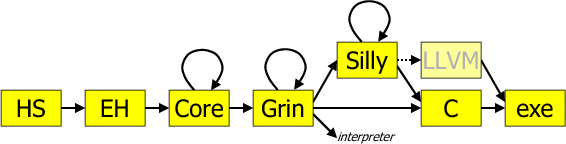
\includegraphics[scale=0.8]{ehc-dataflow2}
\caption{UHC pipeline}
\label{flow}
\end{figure}

For this thesis only the first two phases are interesting. The HS and the EH phase are reused:
\begin{description}
\item[\textbf{HS}] This phases is to parse the concrete Haskell syntax into the abstract syntax. 
\item[\textbf{EH}] The Haskell syntax contains a lot of syntactic sugar. In the EH phase the abstract syntax is desugared and preprocessed.
\end{description}
\subsection{Variant}
UHC as mentioned before is a series of smaller compilers. These different versions of the compiler are called \emph{variants}. A tool called \emph{shuffle} is used to weave these variants together. The variant used in this thesis is variant 8. This variant provides no code generation but does provide a parser, renamer, desugarer and typechecker which we can over write.

In terms of \emph{Haskell98} all the needed constructs are there except for \emph{type classes}. This variant is simple enough to be implemented in the alloted time, but complete enough that we can implement a large subset of Haskell functionality using it. Including higher-rank functions.

\subsection{EH}
The abstract language used by the Utrecht Haskell Compiler (UHC) to represent desugared Haskell is called Essential Haskell or EH for short. EH at it's core resembles $\lambda-calculus$ but with added \textbf{Let} bindings. EH represents a Haskell file but with all the syntactical sugar of the HS file removed, leaving only a core set of basic operations that need to be supported.


\chapter{Attribute Grammars}
\emph{Context Free Grammars}(CFG) cannot describe the complete syntax of programming languages\cite{knuth1}, particularly specifying any context-sensitive condition is impossible. For example the condition that the same value for \emph{n} be enforced in the string $a^nb^nc^n$ cannot be tested by using context free grammars\cite{ken}.

Developed in 1968 by Donald E. Knuth \ags were created as a way to define \emph{meaning} to context free languages. An example of assigning meaning to a grammar would be defining the evaluation of expressions defined by the following \emph{CFG} expressed as \emph{BNF}:

\begin{figure}[H]
\begin{grammar}
      [(colon){$\rightarrow$}]
      [(semicolon)$|$]
      [(comma){}]
      [(period){\\}]
      [(quote){\begin{bf}}{\end{bf}}]
      [(nonterminal){$\langle$}{$\rangle$}]
<Expr>   \hspace{52pt} : <number>; <Expr>, <operator>, <Expr>.
<number> \hspace{42pt} : <digit>;<digit>,<number>.
<digit> \hspace{55pt} : "0";"1";"2";"3";"4";"5";"6";"7";"8";"9".
<relational operator>: "$-$";"$+$".
\end{grammar}
\caption{BNF definition for Expressions}
\label{grammar:bnf:expr}
\end{figure}

The \emph{terminals} in this case are the \emph{operators} $+,-$ and the \emph{digits} $0\ldots 9$. The \emph{nonterminals} are the \emph{Expr} and \emph{number} symbols. The grammar specifies that an expression is either a \textbf{number} or an \textbf{Expr} followed by an \textbf{operator} and then another \textbf{Expr}. For every sentence that can be produced by this grammar a parse tree can be assigned. For instance the expression "2 + (3 - 5) + (6 - 1)" produces the parse tree in figure \ref{fig.example1.parsetree}. Meaning is defined for the expression on a step by step basis corresponding with the structure of the parse tree, starting from the leaves and working up the tree. This is done by assigning \emph{attributes} to the tree.

\begin{figure}[H]
\centering
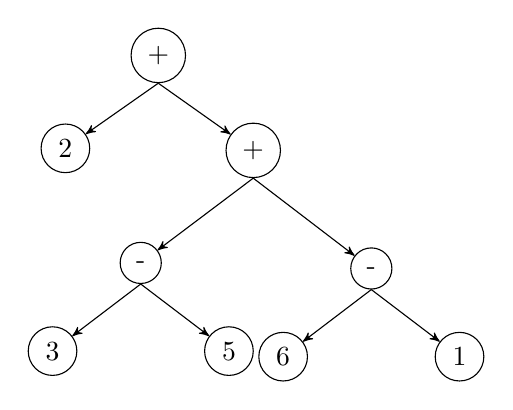
\begin{tikzpicture}[>=stealth']
\node (r0) [draw, circle] {+};
\node (r1) [below left=1cm of r0, draw, circle] {2}
  edge[<-] (r0.south);
\node (r2) [below right=1cm of r0, draw, circle] {+}
  edge[<-] (r0.south);
\node (s0) [below left=1.4cm of r2, draw, circle] {-}
  edge[<-] (r2.south);
\node (s1) [below left=1cm of s0, draw, circle] {3}
  edge[<-] (s0.south);
\node (s2) [below right=1cm of s0, draw, circle] {5}
  edge[<-] (s0.south);
\node (f0) [below right=1.5cm of r2, draw, circle] {-}
  edge[<-] (r2.south);
\node (f1) [below left=1cm of f0, draw, circle] {6}
  edge[<-] (f0.south);
\node (f2) [below right=1cm of f0, draw, circle] {1}
  edge[<-] (f0.south);
\end{tikzpicture}
\caption{Parse tree example for "2 + (3 - 5) + (6 - 1)"}
\label{fig.example1.parsetree}
\end{figure}

AG's are additions to CFGs that propagate semantic information along through parse trees. As with the majority of trees used in computer science, ASTs are created with the \emph{root} at the top and the \emph{leaves} at the bottom. With this in mind there are two kinds of \emph{attributes} defined by knuth\cite{knuth1}:
\begin{description}
\item[\textbf{synthesized}] An attribute that is only dependent on \emph{descendants} of the nonterminal. They are passed bottom-up through the tree.
\item[\textbf{inherited}] An attribute that is defined in terms of the \emph{ancestors} of the nonterminal. They are passed top-down through the tree.
\end{description}

An attribute can be both \emph{synthesized} and \emph{inherited}. Semantics can be defined for the tree in figure \ref{fig.example1.parsetree} by assigning a \emph{value} synthesized attribute of type \textbf{Int} to the nonterminals \emph{number} and \emph{Expr}. The evaluation rules are:

\begin{figure}[H]
\begin{grammar}
      [(colon){$\rightarrow$}]
      [(semicolon)$||$]
      [(comma){}]
      [(period){\\}]
      [(quote){\begin{bf}}{\end{bf}}]
      [(nonterminal){$\langle$}{$\rangle$}] 
value(<$Expr^+$>):value(<$Expr_1$>) + value(<$Expr_2$>). 
value(<$Expr^-$>):value(<$Expr_1$>) - value(<$Expr_2$>). 
value(<Expr>):value(<number>).
value(<number>):<number>.
\end{grammar}
\caption{attribute definition for Expressions}
\label{semantics:bnf:expr}
\end{figure}

Subscripts are used to disambiguate between the different expression types and  superscripts are used to distinguish between the different cases of the \emph{operator} in an expression. Figure \ref{fig.example2.decoratedtree} shows a tree decorated with the synthesized attribute \emph{v} (short for value) along with intermediate values of \emph{v}.

\begin{figure}[H]
\centering
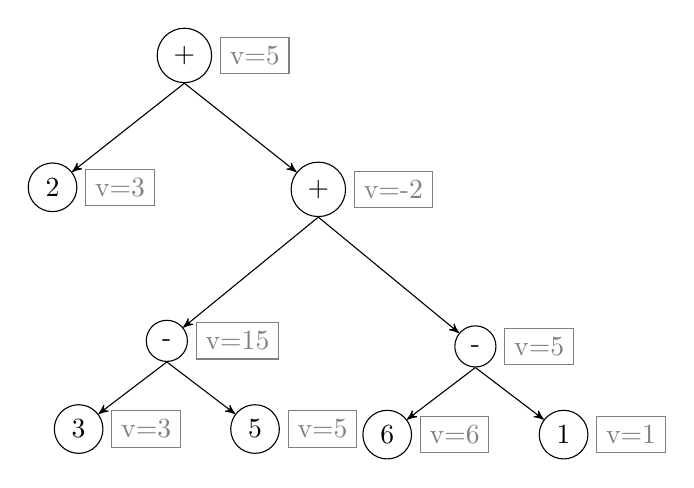
\begin{tikzpicture}[>=stealth']
\node (r0) [draw, circle] {+};
\node (ri0) [draw, rectangle, right=0.1cm of r0, gray] {v=5};
\node (r1) [below left=1.7cm of r0, draw, circle] {2}
  edge[<-] (r0.south);
\node (ri1) [draw, rectangle, right=0.1cm of r1, gray] {v=3};
\node (r2) [below right=1.7cm of r0, draw, circle] {+}
  edge[<-] (r0.south);
\node (ri2) [draw, rectangle, right=0.1cm of r2, gray] {v=-2};
\node (s0) [below left=2.1cm of r2, draw, circle] {-}
  edge[<-] (r2.south);
\node (ri3) [draw, rectangle, right=0.1cm of s0, gray] {v=15};
\node (s1) [below left=1.0cm of s0, draw, circle] {3}
  edge[<-] (s0.south);
\node (ri4) [draw, rectangle, right=0.1cm of s1, gray] {v=3};
\node (s2) [below right=1.0cm of s0, draw, circle] {5}
  edge[<-] (s0.south);
\node (ri5) [draw, rectangle, right=0.1cm of s2, gray] {v=5};
\node (f0) [below right=2.2cm of r2, draw, circle] {-}
  edge[<-] (r2.south);
\node (ri6) [draw, rectangle, right=0.1cm of f0, gray] {v=5};
\node (f1) [below left=1.0cm of f0, draw, circle] {6}
  edge[<-] (f0.south);
\node (ri7) [draw, rectangle, right=0.1cm of f1, gray] {v=6};
\node (f2) [below right=1.0cm of f0, draw, circle] {1}
  edge[<-] (f0.south);
\node (ri8) [draw, rectangle, right=0.1cm of f2, gray] {v=1};
\end{tikzpicture}
\caption{decorated tree example for "2 + (3 - 5) + (6 - 1)"}
\label{fig.example2.decoratedtree}
\end{figure}

\Ags are akin to \emph{catamorphisms}, except without the need to define the algebra and explicit traversals of the tree.

\section{Utrecht University Attribute Grammar Compiler (UUAGC)}
UUAGC (Utrecht University Attribute Grammar Compiler) is a preprocessor which parses Attribute Grammars in a custom language.
It defines ways to specify an AST, attributes for the terminals and nonterminals and the semantic functions. It is used in the Utrecht Haskell Compiler to do most of the work.

\subsection{Limits of UUAGC}
The \emph{UUAGC} system has a limitation in that it can't perform case distinctions over multiple \emph{abstract syntax trees} at the same time\cite{visitag}. For most applications this is not an issue, since in most cases there is only one \emph{AST} that needs to be traversed at a time. 

Unification is the act of trying to find structural \& semantic equivalence between two types. It is a critical part of type checking, given two types \emph{$t_{1}$} and \emph{$t_{2}$} unification attempts to find a list of substitutions that allows the instantiation of type \emph{$t_{1}$} to type \emph{$t_{2}$}. For this to be accomplished it needs to be possible to traverse both \emph{$t_{1}$} and \emph{$t_{2}$} concurrently while comparing the types at every node.

%\begin{figure}[!h]
%\begin{center}
%\begin{neatopic}[width=.5\textwidth, height=50mm]
%    subgraph type1 {
%	  node [];
%	  a1 [label="a"];
%	  a2 [label="b"];
%	  a1 -- a2;
%	  label = "Type 1";
%    }
%
%    subgraph type1 {
%	  node [];
%	  b1 [label="Int"];
%	  b2 [label="Int"];
%        b1 -- b2;
%	  label = "Type 2";
%    }
%    
%    {rank=same; a1 b1}
%    {rank=same; a2 b2}
%
%    a1 -- b1 [style=dotted, label ="a:= Int"];
%    a2 -- b2 [style=dotted, label ="b:= Int"];
%\end{neatopic}
%\end{center}
%\caption{Unification example}
%\label{unify-simple}
%\end{figure}

When unifying the type \emph{$a \rightarrow b$} with \emph{$Int \rightarrow Int$} both trees are traversed concurrently while the nodes are compared and ultimately terminating with the substitution list [(a,Int), (b, Int)]. The ability to be able to traverse \emph{AST}s that were just produced is also required because the structure of the \emph{type} being produced is not known a priori. During type inference more type information is gradually gained on the type that needs to be produced. This generally presents a problem for AGs\cite{ruler-front} because the synthesis and evaluation phases are two separate passes.

\section{Ruler-Core}
Ruler-core addresses these restrictions in AG by introducing a model based on \emph{visit}\cite{visits} functions. The resulting language is more flexible while still retaining the core semantics of reasoning over decorated trees with attributes. The simplest description of ruler-core would be:\emph{a language to manipulate visit sequences.}

\begin{quotation}
A \emph{visit function}\cite{visitag} is a (partial) function that takes several inputs (\emph{inherited attributes}) and produces several output values (\emph{synthesized attributes}).
\end{quotation}

As with traditional AGs \emph{inherited}, attributes are passed top-down in the tree while \emph{synthesized} attributes are passed bottom-up. An attribute can be both \emph{synthesized} and \emph{inherited}.

Everything that can be expressed in uuagc can be expressed in ruler-core, but the inverse is not true. One of the simplest things that can be done in ruler-core is the evaluation of a single AST. In order to write an evaluator for the expression type in figure \ref{grammar:bnf:expr} we first need to define the \emph{datatypes} and \emph{interfaces}.

\begin{figure}[H]
\begin{minipage}[t]{0.4\linewidth}
\begin{code}
data Expr
  con Num
    val     :: Int
  con Expr
    exp1    :  Expr
    op      :: Operator
    exp2    :  Expr
\end{code}
\end{minipage}
\begin{minipage}[t]{0.6\linewidth}
\begin{code}
data Operator
  con Plus
  con Minus

itf Expr
  visit eval
    inh ast :: Expr -- input
    syn v   :: Int  -- output
\end{code}
\end{minipage}
\caption{Evaluating expressions in ruler-core: datatypes}
\label{example:tutorial1:datatypes}
\end{figure}

\subsubsection{Data types}
\Rcore data types resemble Haskell's record syntax with some notable differences.

Instead of an $=$ or \textbar \space like in Haskell, an explicit \textbf{con} keyword is used to indicate the \emph{name} of the constructor. Every element of the constructor must be explicitly named. Indentation is also important since indentation separates constructors, in general \textbf{con} should be deeper indented then \textbf{data} and the members of a constructor should be indented further than the \textbf{con}. 

Figure \ref{example:tutorial1:datatypes} illustrated two different ways of declaring a type of constructor argument. $:$ is used to declare a type that is a \emph{nonterminal} and $::$ indicates a \emph{terminal}. The reason for this distinction is that for \emph{nonterminal} some extra machinery is defined, it is important to know that for every nonterminal \rcore enforces that at least one of the declared visits have an \emph{inherited} attribute named \emph{ast} with the type of the datatype for which a semantic function is to be defined (more on this later).

Only types of kind $:: \star$ are allowed by \rcore, which means only monomorphic types are accepted. As with UUAGC the constructors generated will be in the form of \emph{TypeName\_ConstructorName}. To put this concretely figure \ref{example:tutorial1:datatypes} exposes for the type \emph{Expr} the constructor functions \textbf{Expr\_Num} and \textbf{Expr\_Expr}.

\subsection{Interfaces}
\emph{Interfaces} are analogous to the interface definitions in other languages, except instead of declaring function prototypes/signatures we declare visits and their attributes. Interfaces declare \emph{Non-Terminal}s which can be named the same as their corresponding \emph{data types}. For those familiar with uuagc, a \textbf{ATTR} declaration in uuagc would equal an interface declaration with one visit and all the attributes declared in the \textbf{ATTR} would be part of this one visit. The ability to explicitly declare these visits and interfaces is where ruler-core's true abilities come in.

\begin{figure}[h!]
\begin{code}
itf <name>
  {visit <name>
    {attributes}
  }
\end{code}
\caption{Ruler-core interface declaration syntax}
\label{itf:syntax}
\end{figure}

As many visits as needed can be declared inside an interface. Every visit is a new \emph{co-routine} and will be scheduled to run by ruler-core. Visits are usually executed as soon as possible and as many visits as possible are executed at the same time. % Outside of visits we can also declare attributes. These attributes are thus not explicitly assigned to a visit. They will be automatically assigned to the earliest visit possible.

\subsection{Visits}
Visits are co-routines (functions) that can be invoked to perform a computation, the synthesis of attributes are done in these sequential passes. Visits consist of different clauses. If a visit only has one clause, it does not have to be declared. 

Visits like all functions have arguments, or in this case attributes. The \emph{inh} keyword indicates an \emph{inherited} attribute (input value) whereas the \emph{syn} indicates a \emph{synthesized} attribute (output value). The order of declaration of the attributes are not important.

After declaring the datatypes and interfaces, the actual semantic function can be declared to evaluate the expressions:

\begin{figure}[H]
\begin{code}
datasem Expr
   clause Num
     lhs.v = loc.val -- output
   clause Expr
     internal opcheck
       clause Plus
         match Operator.Plus@loc = loc.op
         lhs.v = exp1.v + exp2.v -- output
       clause Minus
         match Operator.Minus@loc = loc.op
         lhs.v = exp1.v - exp2.v -- output
\end{code}
\caption{Evaluating expressions in ruler-core: datasem}
\label{example:tutorial1:datasem}
\end{figure}

Figure \ref{example:tutorial1:datasem} has various elements that can be best explained in isolation. Keep this figure in mind when reading.

\subsection{Semantic functions}
\label{semantics}
Semantic functions are used to define semantics interfaces. Within a semantic function it is possible to \emph{invoke} any other coroutine(s) that might be needed. Although there is an implicit \textbf{invoke} keyword it is rarely needed to explicitly \emph{invoke} a visit. When all attributes are defined for a visit it is implicitly invoked.

Within a semantic function it is possible to have any number of semantic rules. Clauses provide a way to do scoping. A clause inherits all the attributes of its parent clauses in the same visit. If a visit has only one clause it doesn't have to be explicitly declared. 

There are two ways of defining a semantic function: using the \textbf{datasem} and a \textbf{sem} keyword. The example in figure \ref{example:tutorial1:datasem} uses the former.

\subsubsection{Datasem}
Defining semantics for a \emph{data type} and \emph{nonterminal}(interface) defined in \rcore can be done with a shorthand: \textbf{datasem}. As the name suggests \textbf{datasem} stands for \emph{datatype semantics}. Those familiar with uuagc can compare defining a \textbf{datasem} in \rcore with a \textbf{SEM} declaration in uuagc.

\begin{figure}[!h]
\begin{code}
datasem <nonterminal> [monad <type>]
    {clause <name>
        ...
    }
\end{code}
\caption{Syntax definition of a sem function}
\label{datasem:syntax}
\end{figure}

Defining a \textbf{datasem} is a shorthand for defining a \textbf{sem} (more on this later). The \emph{monad} type does not need to be specified, however if a type was specified for any semantic function which is used by, or used in this \textbf{datasem} then to disambiguate you need to define the type in this declaration as well.

The \emph{clauses} in a \textbf{datasem} should coincide with the constructors of the data type. The preprocessor enforces that there is a clause for every declared constructor. Every clause declaration implicitly adds a \textbf{match} statement for every clause. This is the reason why there is a required attribute \emph{ast} for ever nonterminal. This is the attribute on which matches are tried out on in the main clauses of a \textbf{datasem}. A \textbf{match} is essentially an assertion, if failed nothing else for that clause is tried out and backtracking takes place.

For every \textbf{datasem}, in every clause where there is a nonterminal in the definition of that clause, there will be an implicit child declared for that field. It is for this reason that in figure \ref{example:tutorial1:datasem} it is refered to the operator terminal via the local child (loc.op) and the \emph{exp1} and \emph{exp2} nonterminals directly. In the case of \emph{Expr} there was only one \emph{inherited} attribute: ast, but since ast is filled in automatically by \rcore the invoke is implicitly performed. Which is why the synthesized attributes can be accessed without any further action. 

\subsection{Bindings}
\label{bindings}
In Haskell the \emph{Let} binding is used when introducing new variables in a sequential computation. In \rcore the keyword \textbf{let} is not used when assigning values to bindings, however since bindings in \rcore are translated to \textbf{let} declarations by the preprocessor the same behaviors is to expected. This means that binding to a \emph{pattern} on the \emph{left hand side} is valid. e.g. \[ (\alpha, \beta) = \ldots \] is allowed. This allows the definition multiple attributes at the same time.

While it is possible to read any attribute as many times as needed, assignment of values to a visits attributes are only allowed once per visit. The compiler will generate an error if it finds code that tries to redefine an attribute (there is no shadowing).

The notation for referencing patterns, expressions and variables is \emph{k}.\emph{x} where \emph{k} is the name of child name and \emph{x} the attribute to be referenced. There are two build in reserved children:

\paragraph{lhs}
The \emph{lhs} child is used to access the \emph{inherited} attributes and to assign values to the \emph{synthesized} attributes. Which one is intended is derived from the context in which they are used: When used at the \emph{left hand side} of an expression they are treated as \emph{synthesized} attributes but when used in the \emph{right hand side} of a binding they refer to the \emph{inherited} values.
 
\paragraph{loc}
The \emph{loc} child is used in a way that is analogous to local variables in other languages. You can define as many of these as needed. The scope of the \emph{loc} is only the clause/visit that it's declared in and it's children.


\subsection{Clauses}
Clauses are a way of defining alternatives. When an assertion in clause fails  it backtracks out of the clause and the next one is tried out. Clauses are tried out in sequential order. A visit can contain multiple clauses, corresponding to the different ways to interpret the \emph{inherited} attributes of the visit.

If no clause can be executed in a visit, the system backtracks to the parent visit and clause. This behavior goes all the way up to the root. In order to be able to generate proper errors it is recommended to always make the collection of clauses for a visit total. The easiest way to do this is to make a \emph{catch-all} clause at the end.

\subsection{Matches}
Matches are akin to case expressions, like case expressions they force evaluation and attempt to pattern match on the constructor. For any data type defined in \rcore itself and the \emph{Bool} type a \textbf{match} can be done.

\begin{figure}[h!]
\begin{code}
match TypeName.ConstructorName@child  = <expression>
\end{code}
\caption{Match syntax definition}
\label{match:syntax}
\end{figure}

If the \emph{match} succeeds the \emph{named} attributes defined for the elements of the Constructor are added as attributes of the specified \emph{child}. Of the two reserved children \textbf{lhs} and \textbf{loc} only \textbf{lhs} is not allowed as a child name here\footnote{note that the childname "var" is also reserved, but in the case of var you will get an actual syntax error}. On the other hand if the \emph{match} fails the entire clause is aborted and backtracking is performed.
There are exceptions to this syntax, \emph{build in} types such as \emph{Bool} which have no children have an alternative syntax:

\begin{figure}[h!]
\begin{code}
match True = <expression>
\end{code}
\caption{Example match on Bools}
\label{match:bool}
\end{figure}

Figure \ref{match:bool} shows that on certain types the rules are relaxed, particularly the Bool type. Note that because there is no build in support for the \emph{Maybe} type, often in this thesis this will be supported by first match on True = isJust \emph{expr} and then a subsequent call the \emph{fromJust} function.

\subsection{Internal}
Sometimes it is necessary to make a decision inside a clause to branch. For example on a value that was just synthesized. This is achieved by using the \emph{internal} keyword. The \emph{internal} keyword provides a means of scoping and branching at the same time. Internals contain a list of \emph{clauses} which will be tried out in order one at a time. Attributes that were declared before the \emph{internal} statement are all in scope inside an internal block. 

\begin{figure}[h!]
\begin{code}
internal <name>
  {clause}
  {clause}
  ...
\end{code}
\caption{Internal syntax definition}
\label{internal:syntax}
\end{figure}

Unfortunately once branched the execution flow never returns back to the parent clause in question. Any code below the internal is floated upward.

\subsection{Invoking semantic functions}
To complete this example we also need be able to call semantic functions from Haskell:

\begin{figure}[H]
\begin{code}
eval :: Expr -> IO Int
eval exp = do
  let inh = Inh_Expr_eval { ast_Inh_Expr = exp }
  syn <- invoke_Expr_eval dnt_Expr inh
  let x = v_Syn_Expr syn
  return x
\end{code}
\caption{calling wrappers from within haskell}
\end{figure}

The first line (the let) defines the \emph{inherited} attributes expected for the visit that is to be called. In this case the "eval" visit, which specified that there is one \emph{inherited} attribute called \emph{ast}. For every visit there is a record for the \emph{inherited} and \emph{synthesized} attributes. The record name is build up as \textbf{X\_I\_v} where \textbf{X} equals "Inh" or "Syn", \textbf{I} is the interface name and \textbf{v} the visit name.

The labels of the fields inside these record are made up of \textbf{attr\_X\_I} where \textbf{attr} is the attribute name, \textbf{X} either "Inh" or "Syn" indicating the attribute type and \textbf{I} the interface name.

The second line invokes the \textbf{eval} routine with the given \emph{inherited} attributes and returns the \emph{synthesized} attribute records. The syntax for invoking a visit is \textbf{invoke\_I\_v \emph{wrapper inhs}}. The \textbf{I} indicates the interface name, the \textbf{v} the visit name, \textbf{inhs} stands for the record containing the inherited attributes and finally \textbf{wrapper} is the wrapper function to call. For every \textbf{datasem} \rcore defines a wrapper \textbf{dnt\_I} and for every \textbf{sem} function the name which was explicitly given is used (more on this later).

The expression example can be scaled up and variables added to expressions. Two extra constructors need to be introduced to \emph{Expr} corresponding to introduction and elimination:	

\begin{code}
  con Var
    nm      :: String
  con Let
    nm      :: String
    exp     :  Expr
    body    :  Expr
\end{code}

In order to be able to evaluate variables an \emph{environment} needs to be passed down through the tree to collect all the variables. We do this by modifying the \emph{interface} of \emph{Expr}. The new \emph{interface} definition is:

\begin{code}
itf Expr
  visit eval 
    inh ast :: Expr
    inh env :: Env
    syn v   :: Int
    syn env :: Env
\end{code}

A new attribute \emph{env} is added which is both a \emph{synthesized} and \emph{inherited} attribute. Strictly speaking the \emph{env} could only be an \emph{inherited} attribute, however both are needed if you want to have access to variables introduced in the left branch in Expr in the right branch.

Now that the type and interface have been extended the next step is to extend the datatype semantics to support the new clauses.

\begin{code}
   clause Var
     loc.val = lookup loc.nm lhs.env
     lhs.v   = fromMaybe (error ...) loc.val
   clause Let
     loc.env  = (loc.nm, exp.v): lhs.env
     body.env = loc.env
     lhs.v    = body.v
\end{code}

The code for \emph{Var} and \emph{Let} show that \emph{lhs} is used both for synthesized and inherited attributes. Which is intended is determined by the way it is used (see section \ref{bindings}).

Sometimes special types such as Lists are needed. The next example shows how list support is provided in \rcore by adding the ability to evaluate a list of expressions.

\subsection{Special types}
At the time of writing \rcore only supports \emph{List}s in this category, but could be easily extended to support any product type like \emph{Maybe} and \emph{Map}.

\subsubsection{Lists}
Lists are declared using the \textbf{type} keyword. The syntax should be very familiar for a Haskell programmer: \[ \textbf{type} \hspace{5pt} \emph{name} : [\emph{type}] \]

Declaring the list type \emph{Expr} would look like:

\begin{figure}[H]
\begin{code}
type Exprs : [Expr]
\end{code}
\caption{Exprs declaration using a list type}
\label{type:exprs}
\end{figure}

Figure \ref{type:exprs} declares the \emph{Non-Terminal} Exprs. This definition could be seen as the data declaration in figure \ref{type:lists}. It introduces  two type constructors \emph{Nil} and \emph{Cons} along with some extra attributes.

\begin{figure}[H]
\begin{code}
data Exprs
  con Nil
  con Cons
    hd : Expr
    tl : Exprs
\end{code}
\caption{Syntactically equivalent definition of the Exprs type}
\label{type:lists}
\end{figure}

Next to creating the syntactic information, ruler-core also generates some \emph{Interface} declarations for every list type. 

The interface declared for the \emph{Exprs} example in figure \ref{type:lists} is equivalent to:

\begin{figure}[h!]
\begin{code}
itf Exprs
  visit exprs_visit
    inh ast :: Exprs
\end{code}
\caption{Ruler-core interface declaration syntax}
\label{itf:exprs}
\end{figure}

A special \emph{inherited} attribute \textbf{ast} is declared on which \emph{matches} will be performed in clauses. This interface itself is not useful, instead the preprocessor enforces that at least one of the visits declared for the \emph{non-terminal} Exprs contain an inherited attribute \emph{ast}. If this is not the case an error will be generated.

With figure \ref{type:lists} and \ref{itf:exprs} in mind the real interface to our \emph{Exprs} type can be declared along with the corresponding \textbf{datasem}.

\begin{figure}
\begin{minipage}[t]{0.4\linewidth}
\begin{code}
itf Exprs
  visit eval 
    inh ast :: Exprs
    inh env :: Env
    syn v   :: [Int]
    syn env :: Env
\end{code}
\end{minipage}
\begin{minipage}[t]{0.6\linewidth}
\begin{code}
datasem Exprs
   clause Cons
     hd.env  = lhs.env
     tl.env  = lhs.env
     lhs.v   = hd.v : tl.v
     lhs.env = lhs.env
   clause Nil
     lhs.env = lhs.env
     lhs.v   = []
\end{code}
\end{minipage}
\end{figure}

A lot of time is spent just copying over the \emph{env} attribute without actually doing anything with it. The larger the program gets the more problematic this becomes. For that \rcore has a special mechanism:

\subsection{Default rules}
Default rules are a way of specifying default values for attributes that will be used in case an explicit values is not given for the attributes in question. This is particularly useful for when it is required to do nothing in some clauses.
When using a \emph{default} rule all the visits of all the children of the current interface become active, which means every \emph{inherited} attribute must be filled in.
These rules are for both \emph{inherited} and \emph{synthesized} attributes. In case an attribute is both then the rule applies to both. 

The values are collected in such a way that they are added to the list in order of occurrence. Meaning the \emph{head} of the list contains the value at the root and the \emph{tail} of the list contains the last value visited. There are two kinds of \emph{default} rules:
\begin{description}
\item[\textbf{default}] { The \textbf{default} keyword gives an error when none of the children of an attribute for which the rule is defined for return a result. }
\item[\textbf{default?}] { The other keyword \textbf{default?} however returns the empty list instead of an exception when no child has the \emph{synthesized} attribute in mention. For \emph{inherited} attributes the value \emph{lhs.attribute} is also added to the list. }
\end{description}

\begin{figure}[h!]
\[
\textbf{default[\textit{?}]} \hspace{5pt} \emph{attribute} = \emph{function}
\]
\caption{Syntax for default expressions}
\label{default:syntax}
\end{figure}

The default rules look at the attribute names and not the types. If a child defines an attribute for which there is a \emph{default} rule defined but where the \emph{type} of this attribute is different then the type of the other element of the list, then a type error will be generated by the Haskell compiler since Haskell lists are heterogeneous.

Using default rules we can simplify the definition of the Exprs datasem:

\begin{code}
datasem Exprs
   default? env = last
   clause Cons
     lhs.v = hd.v : tl.v
   clause Nil
     lhs.v = []
\end{code}

\subsection{Multiple tree traversals}
The previous examples are all possible with uuagc and so with standard attribute grammar, whereas the following example is not. To show how to traverse multiple trees at the same time, and the higher-orderedness of \rcore the following example deals with how to compare two trees for equality.

The interesting points of this example are:
\begin{itemize}
\item Traverse two AST at a time and compare them while evaluating the tree at the same time.
\item While synthesizing the tree, if the tree turns out to be equal return at the same time a new tree with the value at the given node.
\end{itemize}

The easiest one to start with is the \emph{Operator} terminal. An interface that allows the comparison of two operators needs to be defined:

\begin{figure}[H]
\begin{minipage}[t]{0.3\linewidth}
\begin{code}
data Operator
  con Plus
  con Minus
\end{code}
\end{minipage}
\begin{minipage}[t]{0.7\linewidth}
\begin{code}
itf OperatorEq
  visit compare
    inh op1 :: Operator
    inh op2 :: Operator
    syn eq  :: Maybe Operator
\end{code}
\end{minipage}
\caption{Interface to compare two operators}
\end{figure}

The interface \emph{OperatorEq} declares one visit "compare" and within this visit three attributes. The two inherited attributes are the inputs (the two operators to compare) and the synthesized attribute \emph{eq} is the result. The same result pattern will be followed in the rest of the example, if the inputs are equal we return one of the inputs, if not Nothing is returned.

Earlier in section \ref{semantics} it was explained that there are two types of semantic functions. \emph{Data type semantic} functions were explained in that section. This section however requires the second method of implementing semantic functions. The semantic function to compare two Operators is:

\begin{code}
{
eqOp = sem eqOp : OperatorEq monad IO
         visit compare
           default? eq = const False
           clause Plus
             match Operator.Plus@loc = lhs.op1
             match Operator.Plus@loc = lhs.op2
             
             lhs.eq = return Operator_Plus
           clause Minus
             match Operator.Minus@loc = lhs.op1
             match Operator.Minus@loc = lhs.op2

             lhs.eq = return Operator_Minus
           clause other
}
\end{code}

\subsubsection{Sem}
\begin{figure}[!h]
\begin{code}
<name> = sem <internal_name> : <Interface> [monad <type>]
          {visit <name>
             {clause <name>
                ...
             }
          }
\end{code}
\caption{Syntax definition of a sem function}
\label{sem:syntax}
\end{figure}

This method of declaring semantic functions allows the declaration of a semantic function for an arbitrary interface. The different components of figure \ref{sem:syntax} can decomposed as:

%\begin{figure}[ht!]
\begin{description}
\item[\textbf{\textit{name}}] This is the name of a semantic function. It is also the name of the Haskell function that will ultimately be generated for this semantic function. The same naming rules apply as for normal Haskell functions.
\item[\textbf{\textit{internal\_name}}] The internal name is only used internally and is not of real importance for anything done in this thesis.
\item[\textbf{\textit{Interface}}] Interface is the interface for which we are defining a semantic function. Every \emph{synthesized} attribute of the \emph{interface} must be assigned to in the semantic function.
\item[\textbf{monad \textit{type}}] { This is optional. Failure is handled by backtracking. This value specifies the monad to be used while backtracking. This also forces the monad's type from a completely polymorphic type to a more concrete type. The \textit{type} specified should be an instance of \emph{Monad} and \emph{MonadError} due to backtracking of match failures being done by catching errors.}
\item[\textbf{visit \textit{name}}] The name of the visit for which a semantic function is being defined. At least one visit out of the interface should be implemented. Every visit is not required to be implemented, but every \emph{synthesized} attributes should be addressed.
\item[\textbf{clause \textit{name}}] \textit{name} should be a unique name inside the semantic function as the names are used to differentiate the clauses from one another.
\end{description}
%\end{figure}

A \textbf{sem} function does not enforce any kind of condition on visits specified. There is however one important layout rule: every \emph{visit} must be indented at least as deeply as preceding \textbf{sem} keyword. If this is not the case a parse error will be generated.

\subsection{Syntax}
\Rcore like its ancestor \emph{UUAGC} is implemented as a preprocessor for the language Haskell. From a .rul file pure Haskell code, which callable from any other Haskell function is generated. How every bit of the ruler code is translated to Haskell is outside the scope of this thesis but those interested can find it in detail in the paper by Arie Middelkoop\cite{visitag}.

Though it provides various syntactical elements, one of the most important to remember is that the right hand side of an equal sign ($=$) contains Haskell code, which means it is possible to call any Haskell function including library functions from the RHS. 

\subsubsection{Haskell}
In order to \emph{escape} into Haskell mode \emph{curly} braces \{ \} are used. The declaration of a module header and importing Haskell modules can be done with:

\begin{figure}[!h]
\begin{code}
{
{-# LANGUAGE BangPatterns #-}
module Eval where

import Control.Monad.Error
}
\end{code}
\caption{Example Haskell mode escape}
\end{figure}

The location and indentation of the braces do not matter, the code between the braces is copied verbatim to the generated Haskell file. For aesthetic reasons the \emph{curly} braces are usually placed at the beginning of the lines and on a line of their own. 

The next part will show how to compare two expressions, and the declaration of  explicit children in a clause. The place to start is by defining the interface:

\begin{code}
itf Compare
  visit compare
    inh exp1 :: Expr
    inh exp2 :: Expr
    inh env  :: Pair Env
    syn env  :: Pair Env
    syn exp  :: Maybe Expr
\end{code}

\subsection{Children}
One of the benefits of \rcore over traditional AG systems such as \emph{UUAGC} is the ability to synthesize new trees during attribute evaluation. To accomplish this \rcore allows the declaration of new child \emph{non-terminals}. Due to space constrains only a piece of the semantics for the \emph{Compare} interface will be shown. To see the full source please consult the Appendix \ref{appendix:compare}.

\begin{code}
eq = sem eq : Compare monad IO
       visit compare
         default? env = last
         default? exp = const Nothing
         clause Num
           match Expr.Num@e1 = lhs.exp1
           match Expr.Num@e2 = lhs.exp2
           
           loc.eq  = e1.val == e2.val
           lhs.exp = guard loc.eq >> return (Expr_Num e1.val)
         clause Expr
           match Expr.Expr@l = lhs.exp1
           match Expr.Expr@r = lhs.exp2
           
           child left : Compare = eq
           left.exp1 = l.exp1
           left.exp2 = r.exp1
           
           child op : OperatorEq = eqOp
           op.op1 = l.op
           op.op2 = r.op
           
           child right : Compare = eq
           right.exp1 = l.exp2
           right.exp2 = r.exp2
           
           lhs.exp = liftM3 Expr_Expr left.exp op.eq right.exp
\end{code}

Contrary to a \textbf{datasem} there is no real distinction between terminals and nonterminals in a \textbf{sem}. There are no explicit children. If a routine is to be invoked it has to be explicitly declared.

\begin{figure}[h!]
\[
\textbf{child} \hspace{5pt} \emph{name} : Interface \hspace{5pt} [= sem_name]
\]
\caption{child declaration syntax}
\end{figure}

This declares a new \textbf{child} \emph{name} belonging to the nonterminal (Interface) defined by the specified visit\cite{visitag}. By default the co-routine to execute is \emph{id} unless otherwise specified. When invoking a child of a nonterminal for which we defined a datasem the \emph{sem\_name} doesn't have to be defined.

\subsection{Ordering}
The order of statements are largely irrelevant, however \textbf{match} statements will always be executed before any other statement declared beneath them. They are also treated as assertions. However statements and assignments can be in any order, when they are scheduled they will be ordered based on their dependencies. Which is why

\begin{code}
l.e = loc.e
loc.e = m.l
\end{code}

is perfectly valid. Because of the dependence of \emph{l.e} on \emph{loc.e}, \emph{loc.e} will be floated above \emph{l.e}. This dependency resolving will also disallow any cycles inside the dependency graph. Cycles would cause an error to be generated by the preprocessor.


%\chapter{Essential Haskell}

\section{Syntax}

\section{Ordering}

\section{Semantics}


\chapter{HML}
\label{HML}
\section{Introduction}
The majority of type inference systems today are an extension of the  Hindler-Milner (HM)\cite{HM} type system. The HML\cite{HML} type system by Daan Leijen is no different in this regard. It extends the Hindley-Milner type system to add support for first class polymorphism. The HML type system is itself an simplification and at the same time a restricted version of MLF\cite{MLF} while retaining the expressiveness of MLF. The MLF type system is another type system for functional languages which provides impredicative higher-rank polyorphism. However it has a more stringent annotation requirement and more complex type representations then the HML type system. The HML type system in contrast to the MLF type system only uses so called \emph{flexible types} (See section\ref{sec:Types}), which make the system easier to used compared to the  MLF type system.

In the HML type system annotations are only needed on function parameters with a polymorphic type(Another version $HML^F$ allows annotations of Let bindings). Because of this conservative annotation requirement and because HML is an extension of HM any program that is well typed in the Hindley-Milner type system is well typed in the HML type system.

The typing rules are thus very similar to those of the Hindley-Milner type system, where every expression can and is assigned a \emph{most} general type. This is true even with higher rank functions. Furthermore the HML type system is an impredicative type system which is very robust with respect to program transformations. It also has some interesting properties, in particular a Let binding can always be inlined or a shared expression abstracted into a Let. Whenever \emph{$e_1$ $e_2$} is well typed then so are \emph{apply $e_1$ $e_2$} and \emph{revapply $e_2$ $e_1$}. In general this means that HML is insensitive to the order of applications, which is a property that is not true of every type system.

The HML type system is not robust towards $\eta-expansion$ since all polymorphic (higher rank) arguments need to be annotated.

\section{Overview}
The idea is to have the expressiveness of the SystemF type system while having the ease of use of the Hindler-Milner type system. Type inferencing in the SystemF type system is undecidable, for instance inferring the type of:

\begin{code}
poly = \f->(f 1, f 'a')
\end{code}

is impossible. Even though the expressiveness of the SystemF type system does allow a type to be given to this function, it cannot be automatically inferred. Some additional notational help is required from the programmer. As mentioned ealier, in the HML type system the only annotations needed would be on the function parameter that needs a polymorphic type:

\begin{code}
poly = \(f::forall a. a -> a) -> (f 1, f 'a')
\end{code}

Functions and data structures can be used freely without any further annotation.

Consider the following example from the paper\cite{FPH}:

\begin{quotation}
\textit{inc} $\hspace{16.5pt}$ :: Int $\rightarrow$ Int\\
\indent \textit{single} $\hspace{3pt}$  :: $\forall\alpha$. $\alpha$ $\rightarrow$ List $\alpha$\\
\indent \textit{append}  :: $\forall\alpha$. List $\alpha$ $\rightarrow$ List $\alpha$ $\rightarrow$ List $\alpha$\\
\indent \textit{map} $\hspace{10.2pt}$  :: $\forall\alpha\beta$. ($\alpha$ $\rightarrow$ $\beta$) $\rightarrow$ List $\alpha$ $\rightarrow$ List $\beta$ 
\end{quotation}

The following expression type checks just fine in the HML type system:
 \begin{code}
let ids = single id
in  (map poly ids, append (single inc) ids)
\end{code}

But would require \textit{ids} to be two incomparable SystemF types at the same time, namely List (Int $\rightarrow$ Int) and List ($\forall\alpha$. $\alpha$ $\rightarrow$ List $\alpha$). This is where \textit{flexible} types come in, the type of ids can now be described as $\forall(\beta\geq \forall\alpha \rightarrow \alpha).$ List $\beta$, which can be interpreted as "any $\beta$ that is an instance of $\forall\alpha \rightarrow \alpha$ the type List $\beta$ is valid". This can be considered as the most "principle" or general type of that expression. The flexible type of ids can then be instantiated to both of the required types. 

These \textit{flexible} types are the key HML, but flexible types are only allowed on \textit{Let}-bindings (see |poly|) and values of a flexible type cannot be passed as arguments.

The algorithms and typing rules in the paper were designed for a simple lambda-calculus language. To be usable they need to be scaled up to one that works on the specific variant of EH in use. As such, the types and terms reflect this requirement.
\section{Types}
\label{sec:Types}
HML introduces various types, most of which are an extensions of Hindley-Milner types. 

\begin{figure}[H]
\begin{eqnarray*}
\sigma & ::= & c \\ 
       & || & \sigma_1 \hspace{5pt} \sigma_2 \\
       & || & (\sigma) \\ 
       & || & \alpha \\ 
       & || & \forall \alpha . \sigma \\
       & || & \omega
\end{eqnarray*}
\caption{Type expressions}
\label{types}
\end{figure}

The $\sigma$ types are the basic SystemF types. Function applications are expressed by applying the arrow constructor ($\rightarrow$) to its arguments. The $\omega$ type is the \emph{Row} type which is the type of a Tuple:

\begin{eqnarray*}
\omega & ::= & \bot \\
       & || & \sigma ; \omega
\end{eqnarray*}

The type $\omega$ is either nothing ($\bot$) or a type followed by a new tuple.
In the SystemF type system, a \emph{type scheme} is represented as $\forall \alpha$. The HML type system introduces a new definition for \emph{type schemes}:

\begin{figure}[H]
\begin{eqnarray*}
\varphi & ::= & \forall (\alpha \geq \varphi_1). \varphi_2 \\
        & || & \sigma \\
        & || & \bot
\end{eqnarray*}
\caption{Type Schemes}
\label{type-schemes}
\end{figure}

Lambda bound values always have a $\sigma$ type since \emph{flexible types} cannot be passed as arguments, however \emph{Let} bound values can have a \emph{flexible type} $\varphi$.
A \emph{type scheme} $\varphi$ is either a \emph{SystemF} type $\sigma$, the polymorphic $\bot$ value or the quantified type $\forall (\alpha \geq \varphi_1). \varphi_2$. A $\varphi$ with a quantified bounds can be instantiated to any instance of it's bounds. Since $\bot$ can be instantiated to anything, the bounds $(\alpha \geq \bot)$ is called the unconstrained bounds. This bounds is also equivalent to the \emph{SystemF} type $\forall \varphi$. The bounds of a \emph{type scheme} can be anything, even types that cannot be instantiated to anything else. An example of such a type is $(\alpha \geq Int).\alpha$, $Int$ cannot be instantiated to anything. Such types are called \emph{trivially quantified} or more specifically such types have a \emph{trivial bounds}.

The dual of this is a scheme with a \emph{non-trivial bounds}. This type is called the \emph{quantified scheme} $\hat{\varphi}$:

\begin{figure}[H]
\begin{eqnarray*}
\hat{\varphi} & ::= & \forall (\alpha \geq \hat{\varphi_1}). \varphi_2 \hspace{5pt} with \hspace{5pt} \alpha \in ftv(\varphi_2) \\
              & || & \bot
\end{eqnarray*}
\caption{Quantified Schemes}
\label{quantified-schemes}
\end{figure}

Even though quantified schemes are presented as a type, they are regarded in this implementation as a type synonym to normal type schemes. The reason is that quantified schemes are just a restriction on a normal type scheme. Treating them the same is safe to do by adding an extra condition to every function that can extend the prefix: \emph{Any function that extends the prefix must not allow a trivial bound to be added}.
The HML type system defines an extra environment called a \emph{Prefix} which holds the quantified bounds of types:

\begin{figure}[H]
\begin{eqnarray*}
Q ::= \alpha_1\geq\hat{\varphi}_1,\ldots,\alpha_n\geq\hat{\varphi}_n
\end{eqnarray*}
\caption{Prefix}
\label{Prefix}
\end{figure}

The prefix cannot contain any trivial bounds, which is why the \emph{Quantified schemes} type $\hat{\varphi}$ is used inside the Prefix $Q$. The domain of the prefix (dom $Q$ = ${\alpha_1 \ldots \alpha_n}$) and the domain of the substitution environment are disjoint. In other words, a type variable is either bound by the prefix or has been substituted away. A type scheme ca either be quantified by itself or quantified by the prefix environment, when any conflicts arise quantifying in the prefix takes precedence.

The next two types are the \emph{monomorphic} $\tau$ type and the \emph{unqualified type} $\rho$. The \emph{monomorphic} type $\tau$ is the same type as in the Hindley-Milner type system, and the \emph{unqualified} $\rho$ type is represents types without any quantifiers. 

\begin{eqnarray*}
\tau  ::= \alpha \hspace{3pt} || \hspace{3pt} (\tau) \hspace{3pt} || \hspace{3pt} c \hspace{3pt} || \hspace{3pt} \tau_1 \hspace{5pt} \tau_2 \\
\rho  ::= \alpha \hspace{3pt} || \hspace{3pt} (\rho) \hspace{3pt} || \hspace{3pt} c \hspace{3pt} || \hspace{3pt} \rho_1 \hspace{5pt} \rho_2
\end{eqnarray*}

Aside from these types there are some syntactic sugar used in the paper and the rest of this chapter:
\label{syntax}

\begin{eqnarray*}
\forall \alpha & ::= & (\forall \alpha \geq \bot) \\
Q.\varphi & ::= & \forall(\alpha_1 \geq \hat{\varphi}_1). \ldots \forall(\alpha_n \geq \hat{\varphi}_n . \varphi
\end{eqnarray*}

This example shows how a Prefix $Q$ is desugared (interpreted) when used as the bounds of a type scheme.
 
\section{Typing rules}
The typing rules in the HML type system are almost the same as the ones in the Hindley-Milner type system, except that in the presence of \textit{flexible types} the \emph{Instantiation} rule is slightly different. Every rule also has an explicit \textit{Prefix} environment. The prefix $Q$ contains the bounds over the \emph{free} variables in $\Gamma$, e, $\varphi$.

\begin{prooftree}
		\AxiomC{$x : \varphi \in \Gamma$}
	\LeftLabel{Var:\quad}
		\UnaryInfC{$Q,\Gamma\vdash x : \varphi$}
\end{prooftree}

The var rule is still very straight forward, if there is a binding for x in the environment $\Gamma$ with the type $\varphi$ then return the type of $\varphi$ for x under the same environment $\Gamma$ and prefix $Q$.

\begin{prooftree}
		\AxiomC{$Q,\Gamma\vdash e : \varphi_1 \quad Q \vdash \varphi_1 \sqsubset \varphi_2$}
	\LeftLabel{Inst:\quad}
		\UnaryInfC{$Q,\Gamma\vdash e : \varphi_2$}
\end{prooftree}

The instantiation rule states that we can always use a instance of a type under the prefix $Q$ as the type of the expression. This instance of relation is denote by the $\sqsubset$ relation above which states that $\varphi_2$ is an instance of $\varphi_1$ under the prefix $Q$

\begin{prooftree}
		\AxiomC{$(Q, \alpha \geq \hat{\varphi}_1), \Gamma \vdash e : \varphi_2 \quad \alpha \notin ftv(\Gamma)$}
	\LeftLabel{Gen:\quad}
		\UnaryInfC{$Q,\Gamma \vdash e : \forall(\alpha \geq \hat{\varphi}_1) . \varphi_2$}
\end{prooftree}

The generalization rule generalizes a type by moving its bounds out from the prefix $Q$ into the type $\varphi$.

\begin{prooftree}
		\AxiomC{$Q,\Gamma \vdash e_1 : \sigma_2 \rightarrow \sigma \quad Q,\Gamma \vdash e_2 : \sigma_2$}
	\LeftLabel{App:\quad}
		\UnaryInfC{$Q,\Gamma \vdash e_1 \hspace{3pt} e_2 : \sigma$}
\end{prooftree}

The application rule is the standard application rule over types. It requires that the type of $e_2$ be equal to the type of the argument of $e_1$. Note that this ranges over normal SystemF type and not type schemes. Type schemes can still be typed using this rule as a type scheme can be present in the bounds of the types $e_1$ and $e_2$ (See \emph{Fun} rule).

\begin{prooftree}
		\AxiomC{$Q,\Gamma \vdash e_1 : \varphi_1 \quad Q,(\Gamma, x : \varphi_1) \vdash e_2 : \varphi_2$}
	\LeftLabel{Let:\quad}
		\UnaryInfC{$Q,\Gamma \vdash \textbf{Let} \hspace{3pt} x = e_1 \hspace{3pt} \textbf{in} \hspace{3pt} e_2 : \varphi_2$}
\end{prooftree}

The Let rule is rather straight forward, given an expression $e_1$ with type $\varphi_1$ and a variable $x$ which in the environment $\Gamma$ has the same type $\varphi_1$ and an expression $e_2$ with type $\varphi_2$ we can create a let binding \textbf{Let} x = $e_1$ \textbf{in} $e_2$.

\begin{prooftree}
		\AxiomC{$Q, (\Gamma, x : \tau) \vdash e : \sigma$}
	\LeftLabel{Fun:\quad}
		\UnaryInfC{$Q, \Gamma \vdash \lambda x. e : \tau \rightarrow \sigma$}
\end{prooftree}

The Fun rule restricts the type of the parameter to a monomorphic type $\tau$ in order to avoid having to guess polymorphic types. This does not mean that a polymorphic type can not be inferred since the type schemes are hidden in the prefix $Q$.

\begin{prooftree}
		\AxiomC{$Q, (\Gamma, x : \sigma_1) \vdash e : \sigma_2$}
	\LeftLabel{Fun-Ann:\quad}
		\UnaryInfC{$Q, \Gamma \vdash \lambda(x :: \sigma_1). e : \sigma_1 \rightarrow \sigma_2$}
\end{prooftree}

The Function Annotation rule provides a mechanism to explicitly annotate abstraction variables with a (possibly) polymorphic type. Like the annotation of the \textit{poly} example above with the needed higher-rank type.

In particular the \textit{FUN} rule for lambda expressions restrict the type of the parameters to be a mono type $\tau$ since any scheme on the mono type is in the Prefix $Q$. Doing so makes it that the types hidden in the Prefix cannot be directly compared to other types. Instead they have to be instantiated as a means of comparison, as oppose to being unified. This is the secret behind the HML type system.  

\section{Semantics}
\subsection{Type scheme}
The semantics of a type scheme ($\br{\varphi}$) is defined by the literature\cite{HML} as:
\begin{figure}[H]
\begin{eqnarray*}
\br{\bot} & = & \br{\forall\alpha . \alpha} \\
\br{\sigma} & = & \{ \sigma^{'} || \sigma \sqsubseteq_F \sigma^{'} \} \\
\br{\forall(\alpha \geq \varphi_1).\varphi_2} & = & \{ \sigma^{'} || \sigma_1  \in \br{\varphi_1}, \sigma_2 \in \br{\varphi_2}, \\ 
   &\mbox{   }& \mbox{   } \overline{\beta} \# ftv(\forall(\alpha \geq \varphi_1).\varphi_2), \\
   &\mbox{   }& \mbox{   } \varphi^{'} \in \br{\forall\overline{\beta}.\lbrack \alpha := \sigma_1 \rbrack\sigma_2}  \} 
\end{eqnarray*}
\caption{Semantics of a type scheme}
\end{figure}

This definition clarifies that in the type $\forall(\alpha \geq (\forall \beta \geq \bot). \beta \rightarrow ). \alpha \rightarrow \beta$ the $3^{rd}$ $\beta$ is actually unbound. By following this semantic a \emph{type scheme} $\varphi$ can always be converted to a \emph{SystemF} type $\sigma$. It is however important not to do this before type checking is finished or you will lose the flexibility that type schemes offer.

The function |ftype| converts any type scheme to a SystemF type while preserving the semantics.

< ftype(phi) = _ft(_nf(phi))
<    _where  _ft(sigma)                                  =  sigma
<            _ft(bot)                                    =  bot
<            _ft(forall (alpha >= bot) . phi)            =  forall alpha . _ft(phi)
<            _ft(forall (alpha >= forall Q . rho). phi)  =  _ft(forall Q . lbrack alpha := rho rbrack phi)           

\subsection{Prefix}
The semantics of the prefix $Q$ written as $\br{Q}$  is defined as the set of SystemF substitutions that can be attained by the domain of the prefix:

\begin{eqnarray*}
\br{\emptyset} & = & \{\lbrack\rbrack\} \\
\br{Q, \alpha, \hat{\varphi}} & = & \{ \theta \textopenbullet \lbrack \alpha := \sigma \rbrack \hspace{5pt} || \hspace{5pt} \sigma \in \br{\hat{\varphi}}, \theta \in \br{Q} \}
\end{eqnarray*}
\subsection{Substitutions}
The substitution environment $\Gamma$ is defined as a list of tuples. Concretely $\Gamma = [(HsName,\varphi)]$. Substitutions are defined as a \emph{type class} in normal Haskell code. The class declaration is

\begin{figure}[H]
\begin{code}
class Apply a where
  app    :: Sub -> a -> a
  appAll :: Env -> a -> a
  appAll env = foldl' (flip (.)) id (map app env)
  
instance Apply a => Apply [a] where
  app s = map (app s)
\end{code}
\label{utils:apply}
\caption{Substitutions}
\end{figure}

The only function that needs to be defined is \emph{app}, which is the application of a substitution. Substitution on an entire environment is given for free by the default definition of \emph{appAll}. 
The substitutions on types is implemented as your standard capture avoiding substitution.
\subsection{Invariants}
For the prefix environment $Q$ and all substitution list $\theta$ there are some restrictions on the ordering of their elements:
\begin{description}
\item[\textbf{$Q$}] The elements in the prefix should always maintain the order of which they were added. Elements are added at the end of the list and are updated in-place. This is important for efficiency reasons since it is known that a particular variable cannot occur in the prefix before the point of its binding. Functions such as Split and Update rely on this.
\item[\textbf{$\theta$}] New elements should always be added in a spot that insures that applying a substitution to a list is a linear operation. To put it differently, elements are inserted at the last position in the list where the co-domain of the substitution and the domain of the preceding elements are disjoint.
\end{description}
\section{Normal form}
During type inferencing it is desirable to bring types into \emph{normal form} in order to make it easier to compare them. It is not a requirement but it simplifies the types and throws away trivial and/or useless quantifications.

Normal form is implemented as another type class:

\begin{code}
class Eq a => Normal a where
  nf :: a -> a
  isNf :: a -> Bool
  isNf x = nf x == x
\end{code}

The specification for \emph{nf} is defined as:

\begin{figure}[H]

< _nf(sigma)                          =  sigma
< _nf(bot)                            =  bot
< _nf(forall(alpha >= phi_1). phi_2)  =  _nf(phi_2)                                 _iff  alpha _in ftv (phi_2)
< _nf(forall(alpha >= phi_1). phi_2)  =  _nf(phi_1)                                 _iff  _nf (phi_2)  =  alpha 
< _nf(forall(alpha >= phi_1). phi_2)  =  _nf(lbrack alpha := rho rbrack phi_2)      _iff  _nf(phi_1)   =  rho
< _nf(forall(alpha >= phi_1). phi_2)  =  forall(alpha >= _nf(phi_1)). _nf(phi_2)

\caption{Normal Form}
\end{figure}

This definition of normal form uses \emph{ftv} which means \emph{free type variables}. Most of the cases for finding the ftv of a type are the standard definitions found in literature. The one exception is for type schemes:

< _ftv(forall(alpha >= phi_1). phi_2)
<    =  _ftv(phi_1) cup _ftv(phi_2)  _iff alpha _in _ftv(phi_2)
<    =  _ftv(phi_2)                  _otherwise


If bounds of a type scheme is not used, then its free variables have no impact on the free variables of the type.
\section{Utility functions}
There are a couple of utilities functions which are used often, in this section their specification and implementation are discussed.
\subsection{Split}
The split function is one of the simplest functions. As the name suggests, it is used to split a prefix $Q$ into two based on a list of domains.

\begin{figure}[H]

< split :: (Q, vec alpha) -> (Q,Q)
< split (empty, vec alpha) = 
<    _return (empty, empty)
< ^^^
< split ((Q,alpha >= hat phi), vec alpha)  =  with alpha _in (vec alpha)
<    _let (Q_1, Q_2) = split (Q,(((vec alpha) - alpha) cup ftv(phi)))
<    _return ((Q_1, alpha >= (hat phi)), Q_2)
< ^^^
< split ((Q,alpha >= (hat phi)), (vec alpha))  =  with alpha _notin (vec alpha)
<    _let (Q_1, Q_2) = split (Q, vec alpha)
<    _return (Q_1, (Q_2, alpha >= (hat phi)))

\end{figure}
The notation of $(Q,x)$ means extending $Q$ by adding $x$ to the end while $(Q_1, Q_2)$ is just the tupling of two prefixes.

The function itself is quite simple and works based on the assumption that the domain of the prefix contains no duplicates. The function also maintains the invariant on the ordering within each individual prefixes it produces. The split function is usually used as an way to do \emph{generalization}.

\subsection{Update}
The update function is used to update an existing binding in a prefix. There are two ways to update a prefix. Both return a tuple consisting of a new prefix and a substitution list. These functions have an implicit requirement that the bound to be updated must already exist within the prefix.
\subsubsection{Update based with new bound}
The first way to update a prefix is with a new scheme:


< update(Q, alpha >= phi_2) =
<    _let (Q_0, (Q_1, alpha >= (hat phi_1), Q_2)) = split(Q, ftv(phi_2))
<               _if(nf(phi_2)= rho)
<                   _then  _return ((Q_0, Q_1, lbrack alpha := rho rbrack Q_2), lbrack alpha := rho rbrack)
<                   _else  _return ((Q_0, Q_1, alpha >= phi_2, Q_2), lbrack rbrack)

The steps performed by this function can decomposed as:

\begin{enumerate}
\item{ Split the prefix into two parts ($Q_0, Q_{0'})$ based on the free variables of the new scheme. This is done for two reasons:  
		\begin{itemize}
		\item As a crude check to prevent infinity types. If the |ftv| of $\varphi_2$ contains $\alpha$ the second operation would fail.
		\item Reinforce the invariant. The prefixes that will not be updated are older and are positioned in the front of the list.
		\end{itemize}
     }
\item Split $Q_{0'}$ in place into 3 parts. $Q_1$ contains the schemes before the current binding to $\alpha$. $Q_3$ contains the schemes after the binding to $\alpha$.
\item{ To prevent that a simple bound enter the prefix a check is performed to see if the normal form of the new scheme $\varphi_2$ is an unqualified type. If it is a simple type, we return the a substitution to the type instead of adding it to the prefix, and the substitution is applied to $Q_2$ because due to the ordering of the prefixes it is the only prefix that can contain any reference to $\alpha$.
However if the type is not a simple type then it is added in-place in the prefix and no substitution is returned.
     }
\item In the return statements, the tupling statement is intended to be an implicit concatenation if the elements. 
\end{enumerate}
\subsubsection{Update based on substitution}
The second way to update a prefix is with a substitution. This update always removes the entry from the prefix:

< update(Q, alpha := sigma) =
<    _let (Q_0, (Q_1, alpha >= varphi, Q_2)) = split(Q, ftv(sigma))
<    _return ((Q_0, Q_1, lbrack alpha := sigma rbrack Q_2), lbrack alpha := sigma rbrack)

\subsection{Extend}
The last way to modify a prefix is by extending it with a new entry. This is done with the help of the extend function:

< extend(Q, alpha >= phi) = 
<    _let (Q', phi') = explode Q phi
<            _if  (_nf(phi') = rho)
<                 _then _return (Q', lbrack alpha := rho rbrack)
<                 _else _return ((Q', alpha >= phi'),lbrack rbrack)

Like before, the normal form checks are here to prevent simple types to enter the environment. However there is another type that shouldn't enter the environment here: \emph{types who's normal form is $\bot$ should not enter the prefix}. 

Concretely this means that extending the prefix with e.g. $\beta \geq (\forall(\alpha \geq \bot).\alpha)$ should just return the substitution $\beta := \alpha$. The reason for this is to prevent information loss when types are shared, this will be covered in more detail in the implementation of Applications.

The definition of the \emph{explode} function is quite simple:

< explode :: Q -> phi -> (Q, phi)
< explode Q phi =
<    _if  (_nf(phi) = bot)
<         _then  _let(forall Q_1 . phi_1) = phi
<                _return (Q Q_1, phi_1)
<         _else _return (Q, phi)

The function works by using the syntactic sugar for quantified type schemes (refer to section \ref{syntax} for more details). If the normal form of the type scheme |phi| is $\bot$ then the type scheme and its prefix are returned separately. The function is a more restrictive form of to the following typing rule:

\begin{prooftree}
		\AxiomC{$Q,\Gamma \vdash e : \forall Q_1 . \sigma$}
	\LeftLabel{Explode:\quad}
		\UnaryInfC{$Q Q_1,\Gamma \vdash e : \sigma$}
\end{prooftree}

\section{Modifications}
This section details some modifications made to the standard HML algorithm that should be explained on their own.
\subsection{Promotion}
In the original algorithm for unification, the following semantically equivalent types for \emph{id} are not treated the same:
\begin{eqnarray*}
\forall a. a \rightarrow a \textrm{ and }
(\forall a \geq \bot). a \rightarrow a
\end{eqnarray*}

They do however result in the same SystemF type. This occurs because we want to retain some link back to types that a normal Haskell programmer is used to. But for the implementation of unification there is really no reason why the SystemF type schemes cannot be removed as inputs and only flexible types accepted. All types, with the exception of the inner quantifiers for higher-rank types are promoted to flexible types. The |forall b.| in |forall a. (forall b. b -> b) -> a -> a| is such a type. The promoted type is |(a >= bot). (forall b. b -> b) -> a -> a|.

\begin{code}
embedF :: TyExpr -> TyScheme
embedF = embed id
  where  embed :: (TyScheme -> TyScheme) -> TyExpr -> TyScheme
         embed val (TyExpr_Parens     s) = embed val s
         embed val (TyExpr_Quant  _ a t) = 
           let e = TyScheme_Quant (Scheme_Simple a TyScheme_Bottom)
           in  embed (val . e) t
         embed val e                     = val (TyScheme_SystemF e)
\end{code}

The reason higher-rank quantifiers inside types are not promoted is that it would require a change of the definition of a type scheme. Unfortunately at the moment of discovery time constraints prohibited this.
\subsubsection{Domain}
Because of types being promoted, we end up with types that are a bit more complex in the prefix. Types as 
\begin{equation}
\tau = \beta \geq ((\forall a \geq \bot). a \rightarrow a)
\end{equation}

are now quite common. When we generalize it is common to do so based on the domain of the initial(input) prefix. By promoting types we introduce new type variables that need to be taken in account, if not we might accidentally disregard a \emph{scheme bound} without noticing. 

For that reason the range of the domain needs to be redefined:
\begin{eqnarray*}
dom   &\tau& = \{\beta, \alpha\}\\
codom &\tau& = \{\}
\end{eqnarray*}

\subsection{Renaming}
\label{renaming}

The type HML system does not have support for case expressions and tuples. In those two situation you would want on every lookup of a type constructor to return a fresh type. e.g. the type of $(\lbrack \rbrack, \lbrack \rbrack)$ should is $\forall \alpha \beta . (\lbrack \alpha \rbrack, \lbrack \beta \rbrack)$. Because of this, on every lookup of a constructor we rename every bound variable. In applications, either the function or the argument needs to be alpha renamed when being added to the prefix. This is because when unifying the type of "id id" the type of both id's are the same. Without the renaming we might end up reasoning about the same type variable accidentally.


\chapter{Implementation}
This chapter details the implementation of the typesystem in \emph{ruler-core}. Due to the amount of code tt will be a tutorial style chapter which introduces the pieces in small bits.
\section{Types}
The implementation of the types can be easily derived from those in figure \ref{types}. To simplify some phases of the implementation the type scheme $\varphi$ and the SystemF $\sigma$ are extended to support the sugared syntaxes at the end of section \ref{sec:Types}:

\begin{figure}
\begin{minipage}[t]{0.5\linewidth}
\begin{code}
  con Sugar
     prefix  :: Prefix
     tyExpr  :: TyScheme
\end{code}
\end{minipage}
\begin{minipage}[t]{0.5\linewidth}
\begin{code}
  con Forall
    qu        :: TyQu
    tyVar     :: [HsName]
    tyExpr    :: TyExpr 
\end{code} 
\end{minipage}
\caption{Addition to the $\varphi$ and $\sigma$ types.}
\label{abs:fig:types}
\end{figure}

Along with these two helper functions \emph{sugar} and \emph{desugar} are defined. The implementation of these two functions isn't that interesting however they do hold the property that \emph{desugar . desugar == id}. These two types facilitate the aggregation of quantified values. For instance $\forall \alpha . \forall \beta. \alpha \rightarrow \beta$ can be represented as $\forall \alpha \beta . \alpha \rightarrow \beta$. Doing this minimizes the amount of code needed in the algorithm implementations, by making it easier to in one pattern matching get all the variables the bounded variables.
\subsection{Type Expressions}
The full syntax of the datatype $\sigma$ is:

\begin{figure}
\begin{minipage}[t]{0.5\linewidth}
\begin{code}
data TyQu
  con TyForall
    
data TyExpr
  con Con
    nm        :: HsName
  con App
    func      :  TyExpr
    arg       :  TyExpr
  con AppTop
    tyExpr    :  TyExpr
  con Parens
    tyExpr    :  TyExpr
  con Ann
    ann       :: TyExprAnn
    tyExpr    :  TyExpr
  con Wild
\end{code}
\end{minipage}
\begin{minipage}[t]{0.5\linewidth}
\begin{code}
  con Mono
  con Var
    nm        :: HsName
  con VarWild
    mm        :: HsName
  con Quant
    qu        :: TyQu
    tyVar     :: HsName
    tyExpr    :  TyExpr
  con Forall
    qu        :: TyQu
    tyVar     :: [HsName]
    tyExpr    :  TyExpr    
  con Row
    rowTyExpr :  RowTyExpr
\end{code}
\end{minipage}
\caption{Datatype description of $\sigma$.}
\label{abs:fig:tyexpr}
\end{figure}

Most of these are pretty standard with the exception of \emph{Row} and \emph{AppTop}. The \emph{Row} constructor is used to represent the type of a Tuple, this will be explained later in Chapter \ref{cap:Extensions}. 
The \emph{AppTop} constructor is used purely for pretty printing purposes, in particular when pretty printing Constructor applications. The $(\rightarrow)$ constructor is not treated specially in this version of EH, which means $\alpha \rightarrow \beta$ is encoded as $((\rightarrow \alpha) \beta)$. The \emph{App} found under an \emph{AppTop} is pretty printed differently to show the expected type above.

\section{Inference}
Like any ruler core program, the first step is to define the datatypes needed and the interfaces. Since type inferencing is done on expressions, we first have to introduce the expression data type:

\begin{figure}
\begin{minipage}[t]{0.5\linewidth}
\begin{code}
data Expr
  con IConst
    int           :: Int
  con CConst
    char          :: Char
  con Con
    nm            :: HsName
  con Var
    nm            :: HsName
  con App
    func          :  Expr
    arg           :  Expr
  con Let
    isStrict      :: Bool
    decls         :  Decls
    body          :  Expr
  con Lam
    arg           :  PatExpr
    body          :  Expr
  con AppTop
    expr          :  Expr
  con Parens
    expr          :  Expr
  con TypeAs
    tyExpr        :: TyExpr
    expr          :  Expr
  con DataFields
    dataFieldExpr :: DataFieldExpr
\end{code}
\end{minipage}
\begin{minipage}[t]{0.5\linewidth}
\begin{code}
itf Expr
  visit infer
    inh pre :: Prefix
    inh env :: Gamma
    inh ast :: Expr
    inh exp :: Expr
    inh frs :: Int
    syn pre :: Prefix
    syn sub :: Env
    syn res :: Maybe TyScheme
    syn frs :: Int
\end{code}
\end{minipage}
\caption{Datatype and interface description of the expression type.}
\label{abs:fig:tyexpr}
\end{figure}

The attentive reader would notice that we have defined datatypes but have not defined any structures for \emph{case} statements. This was done intentionally as \emph{case} statements are an extension of the base algorithm, which will be covered in chapter \ref{cap:Extensions}. This version of EH also only has build-in support for the \emph{Int} and \emph{Char} datatypes.

The interface is quite simple, in the \emph{infer} visit we declare the inherited attributes for the Gamma $\Gamma$, the Prefix $Q$ and expression to infer. The \emph{frs} attribute is used in almost every visit to generate fresh variables, if this value is not passed in a certain visit, the results could be disastrous (type clashes). It has the benefit that it makes every variable unique, which makes it easier to track down problems. With the exception of inferring types for variables, every case in the semantics of $\emph{Expr}$ every type returned should be fully generalized.

Before continuing a small explanation of how EH is constructed is in order:

\subsection{Ordering}
Whenever a Haskell file is desugared into a EH file, some reordering is done. In the EH file function,data declarations and type synonyms are always displayed before any function or other entities that uses them. Or alternatively, for every entity (where entity can be anything that refers to another type/function) a node is created and a dependency graph is made, which is then \emph{Topologically sorted}, that is, for every pair of edge \emph{uv} (\emph{u} is used in \emph{v}) \emph{u} comes before \emph{v}. It's worth noting that datatype and type synonym declarations are always put at the top of the file, before the function declarations.

The first obvious question is, what if functions or datatypes have a cyclic dependency. E.g. mutually recursion:

\begin{code}
data Foo = Foo Bar
data Bar = Bar Foo | NoBar

foo = bar
bar = foo
\end{code}

Aside from the fact that the functions foo and bar never terminate, they should however typecheck perfectly fine. For datatypes nothing special needs to be done to make EH support mutual recursion. When processing datatypes we just always add information about the data \emph{Type} before processing the constructors. For binding processing we do the same. The EH syntax for \emph{Let} allows us to bind multiple \emph{Decl} at once. This means, that We will have one \emph{Let} binding both \emph{foo} and \emph{bar} at the same time.

Any Haskell after desugared to EH is turned into one big \emph{Let} statement terminating in either 0 or \emph{main} depending on if an actual main function is defined in the module.

Figure ?? which does not define a main is desugered into:

\begin{code}
let main = 0
in let data Bar  = Bar Foo | NoBar
       data Foo  = Foo Bar
   in let foo = bar
          bar = foo
      in 0
\end{code}

in this case, since \emph{main} is not dependent on anything it is the top level declaration, in every other cases where main is defined it will be put somewhere inside the dependency graph and the top level \emph{Let} will terminate \emph{in} main.
\subsection{Semantics}

This ordering that EH brings to a Haskell module is quite handy, especially for Attribute Grammar code. Attribute Grammar compilers do computations on attributes defined on the nodes of a tree. A Haskell file desugared into an EH file is now a Top-down tree, where the only case that needs some special handling is mutual recursion. 

This makes certain tasks a lot easier, for instance when looking up a value in the environment, if we can't find it, then it's really not defined. there's no need to look any further. If we can't type check a specific node, it also means we don't have to bother trying any of it's children, since they depend on the node that failed type checking.

\subsection{defining the data semantics}
With the explanation of EH out of the way we can incrementally define the data semantics for inference.

\paragraph{header and variables}
Starting out, we can define the case for variable and constants:
\begin{code}
datasem Expr monad IO
    default? sub = const empty
    default? pre = last
    default? frs = last
    default? res = const Nothing
    clause Var
        lhs.res
             = case lookup loc.nm (unGam lhs.env) of
                Just a  -> return a
                Nothing -> error $ "Variable '" ++ show loc.nm ++ "' not in scope"
    clause IConst
       lhs.res = return $ TyScheme_SystemF $ TyExpr_Con $ mkName "Int"
    clause CConst
       lhs.res = return $ TyScheme_SystemF $ TyExpr_Con $ mkName "Char"
\end{code}

The rules for the default rules are quite simple:
\begin{description}
\item[\textbf{sub}] If no substitutions are defined then just return an empty list
\item[\textbf{pre}] If the prefix isn't changed, just return the last value seen
\item[\textbf{frs}] If no new variables were introduces, just return the last value (which should also be the highest value)
\item[\textbf{res}] If no type is infered, return Nothing
\end{description}

In the case of infering the type of a variable, the only thing to do is just lookup the variable in the $\Gamma$. If the value is not found then the variable is undefined and an error is returned. Error reporting is admittedly crude in the type system, but it gives addiquate feedback.

For the Integer (\emph{IConst}) and the Char (\emph{CConst}) cases, just return the \emph{Int} and \emph{Char} constructors respectively.

\paragraph{Constructors}
For any other constructor the name of the constructor is looked up. But as mentioned in section \ref{renaming} constructors are $\alpha-$renamed.

\begin{code}
    clause Con
       loc.res = maybe (error $ "Constructor '" ++ pp loc.nm ++ "' not found") id (lookup loc.nm (unGam lhs.env))
       (loc.res2, lhs.frs, _) = renameBound lhs.frs loc.res
       lhs.res = return loc.res2
\end{code}

\paragraph{Applications}
Typing two expressions is the first part where the code gets a bit complex:

\begin{code}
    clause App
       (loc.a1, loc.frs1) = fresh lhs.frs
       (loc.a2, loc.frs2) = fresh loc.frs1
       (loc.b , loc.frs3) = fresh loc.frs2
       
       func.exp = loc.func
       func.frs = loc.frs3
       func.pre = lhs.pre
       func.env = lhs.env
       
       match True = isJust func.res
       loc.func_res = fromJust func.res
       
       arg.exp = loc.arg
       arg.frs = func.frs
       arg.pre = func.pre
       
       arg.env = appAll func.sub lhs.env
       
       match True = isJust arg.res
       loc.arg_res = fromJust arg.res
       
       loc.temp1 = extend (arg.pre, Scheme_Simple loc.a1 (appAll arg.sub loc.func_res))
       loc.temp2 = extend (fst loc.temp1, Scheme_Simple loc.a2 (loc.arg_res))
       loc.temp3 = extend (fst loc.temp2, Scheme_Simple loc.b  (TyScheme_Bottom))
       
       (loc.q2', loc.e2') = (fst loc.temp3
                            ,(snd loc.temp1) `munion` (snd loc.temp2) `munion` (snd loc.temp3) `munion` func.sub)
       
       child u : Unify = unify
       u.pre  = loc.q2'
       
       u.exp1 = appAll loc.e2' (TyExpr_Var loc.a1)
       u.exp2 = (appAll loc.e2' (TyExpr_Var loc.a2)) `mkArrow` (TyExpr_Var loc.b)
       u.frs  = arg.frs
       
       loc.q3 = u.pre
       loc.e3 = u.sub
       
       (loc.q4, loc.q5) = curry split loc.q3 (domain lhs.pre)
    
       lhs.res = let b = TyExpr_Var loc.b
                     e = appAll (loc.e3 `munion` loc.e2') b
                 in return $ ptype $ desugar $ TyScheme_Sugar loc.q5 (TyScheme_SystemF e)
       lhs.sub = let subs = func.sub `munion` arg.sub
                 in subs `munion` loc.e3
       lhs.pre = loc.q4
       lhs.frs = u.frs
\end{code}

\section{Unification}
\section{Instantiation}
\section{Error handling} 


\chapter{Towards Haskell98}
\subsection{Case expressions}


\chapter{Conclusions}
\section{Ruler-Core}
\section{HML}
\section{Evaluation}
\section{Future Work}
\section{Conclusion}


\printglossaries
\printindex

\appendix

\begin{thebibliography}{9}
\bibitem{UHC}
  Utrecht Haskell Compiler Structure
  \emph{Structure Documentation}
   \url{http://www.cs.uu.nl/wiki/bin/view/Ehc/EhcStructureDocumentation}
\bibitem{uuagc}
  UUAGC
  \emph{"Utrecht Attribute Grammar System"}
   \url{http://www.cs.uu.nl/wiki/bin/view/HUT/AttributeGrammarSystem}
\bibitem{ruler-front}
  Arie Middelkoop, Atze Dijkstra, S.Doatse Swierstra
  \emph{Iterative Type Inference with Attribute Grammars}
  Utrecht University
\bibitem{visits}
  Saraiva, J. A. B. V., Swierstra, S. D.
  \emph{Purely Functional Implementation of Attribute Grammars}
  Utrecht University, Technical report (1999)
\bibitem{visitag}
  Arie Middelkoop, Atze Dijkstra, S.Doatse Swierstra
  \emph{Visit functions for semantics of Programming Languages}
  Utrecht University
\bibitem{Guesses}
  Arie Middelkoop, Atze Dijkstra, S.Doatse Swierstra, Lucilia Camarao de Figueiredo
  \emph{Controlling Non-Determinism in Type rules using First-Class Guessing}
  Utrecht University, Universidade Federal de Ouro Preto
\bibitem{Ruler}
  Atze Dijkstra, S. Doaitse Swierstra 
  \emph{Ruler: Programming Type Rules}
  LNCS FLOPS 2006 proceedings of FLOPS 2006
\bibitem{Monads}
  Arie Middelkoop, Atze Dijkstra, S.Doatse Swierstra
  \emph{Factoring Type Rules Into Aspects}
  Utrecht University
\bibitem{EH}
  Atze Dijkstra
  \emph{Stepping through Haskell}
  ISBN 90-393-4070-6
\bibitem{outsidein}
  Dimitrios Vytiniotis, Simon Peyton-Jones, Tom Schrijvers, Martin Sulzann
  \emph{Modular type inference with local assumptions}
  Microsoft Research, Katholieke Universiteit Leuven, Informatik Consulting Systems AG.
  Submitted to Journal of Functional Programming.
\bibitem{boring}
  Simon Peyton Jones, Dimitrios Vytiniotis, Stephanie Welrich and Mark Shields
  \emph{Practical type inference for arbitrary-rank types}
  Microsoft Research, University of Pennsylvania, Microsoft
\bibitem{FPH}
  Dimitrios Vytiniotis, Stephanie Weirich and Simon Peyton Jones
  \emph{FPH: First-class Polymorphism for Haskell}
  University of Pennsylvania and Microsoft Research
\bibitem{HML}
  Daan Leijen
  \emph{Robust type inference for first-class polymorphism}
  Microsoft Research
\bibitem{odesky}
  Martin Odersky and Konstantin Laufer
  \emph{Putting Type Annotations to Work}
  University of Karlsruhe and Loyola University Chicago
\bibitem{pierce}
  Benjamin C. Pierce and David N. Turner
  \emph{Local Type Inference}
  Indiana University and Technology Transfer Center
\bibitem{knuth1}
  Donald E. Knuth
  \emph{Semantics of Context-Free Languages}
  California Institute of Technology
\bibitem{knuth2}
  Donald E. Knuth
  \emph{The Genesis of Attribute Grammars}
  Stanford University
\bibitem{ken}
  Ken Slonneger and Barry L. Kurtz
  \emph{Formal Syntax and Semantics of Programming Languages: A Laboratory-Based Approach}
  University of Iowa
\bibitem{HM}
  Luis Damas and Robin Milner
  \emph{Principal type-schemes for functional prorgams}
  POPL '82: Proceedings of the 9th ACM SIGPLAN-SIGACT symposium on Principles of programming languages, ACM, pp. 207–212
\bibitem{MLF}
  Didier Le Botlan and Didier Remy.
  \emph{Recasting MLF.}
  Research Report 6228, INRIA, Rocquencourt, BP 105, 78 153 Le Chesnay Cedex, France June 2007
\end{thebibliography}

\end{document}
